\section{Growth of non-axisymmetric modes without the influence of the
  planet}\label{linear1}
In this section, the planet is introduced at $t=20P_0$ and 
its potential switched on over $10P_0$. At $t=30P_0$ we switch off the
planet potential and azimuthally average the surface density, energy
and velocity fields. At this point the planet has carved a partial
gap and the RWI has not yet occured.
 We then perturb the surface density for $r>r_p$ and continue to 
evolve the disc. We impose  sinusoidal perturbations with 
azimuthal wavenumbers $m\in[1,10]$ and random amplitudes within $\pm 0.01$
 times the local surface density. 
This procedure allows us to analyse the growth of 
non-axisymmetric modes associated with the gap, but without
complications from non-axisymmetry arising directly from disc-planet
interaction (i.e. planet-induced wakes). 

Note that these `planet-off' simulations are not linear stability
calculations since the cooling term in our energy equation
restores the initial temperature profile corresponding to $H/r=0.05$,
rather than the heated gap edge. Linear stability calculations and
adiabatic cases will be further discussed in
section~\ref{adiabatic_section}.  


Simulations here employ a resolution of $(N_r,N_{\phi})=(1024,2048)$
with open boundaries at $r=r_\mathrm{in}$ and
$r_\mathrm{out}=25r_\mathrm{in}$. We consider   
cases with $\tilde{\beta}=0.1,1,10$ corresponding to fast, moderate,
and slowly cooled discs. % {\bf boundary condition for these sims?}

\subsection{Gap structure}
%Since stability of the gap is of interest 
We first examine the gap structure formed by planet-disc
interaction as a function of the cooling time. The azimuthally-averaged 
gap profiles are shown in Fig. \ref{intial1D} for varying
$\tilde\beta$. Gaps formed with lower $\tilde\beta$ (faster cooling)
are deeper with steeper gradients at the gap edges. Faster cooling rates also 
increase (decrease) the surface density maxima (minima). However, a
clean gap does not form in this short time period. 
 

Larger $\tilde\beta$ values result in higher disc aspect ratios $h=H/r$,
i.e. higher temperatures. Heating mostly occur at the gap edges
due to planet-induced spiral shocks. Decreasing the cooling time
implies that this heat is retained in the disc. In the inviscid limit the gap
opening condition is $r_h\gtrsim H$ or $q\gtrsim 3h^3$
\citep{crida06}. 
This indicates that for hotter discs (higher
$h$), it becomes more difficult for a planet of fixed $q$ to open a
gap. This explains the shallower gaps in surface density when
$\tilde{\beta}$ is increased. 
%However, notice the gap structure
%changes most significantly for $\beta =0.1 \to 1.0$. For $\beta \geq
%1$  

The important consequence of a heated gap edge is that the
generalised vortensity profiles, $\tilde{\eta}$, becomes smoother with increasing
cooling times, with the extrema becoming less pronounced. Previous locally
isothermal disc-planet simulations show the RWI associated with PV
minima \citep{li05,lin10}. We can therefore expect the RWI to be associated with
minima in the generalised vortensity (corresponding to local surface
density maxima) in the non-isothermal case. Because the extrema are
less sharp, the RWI is expected to be weaker and the gap to be more
stable with longer cooling times.  

\begin{figure}
  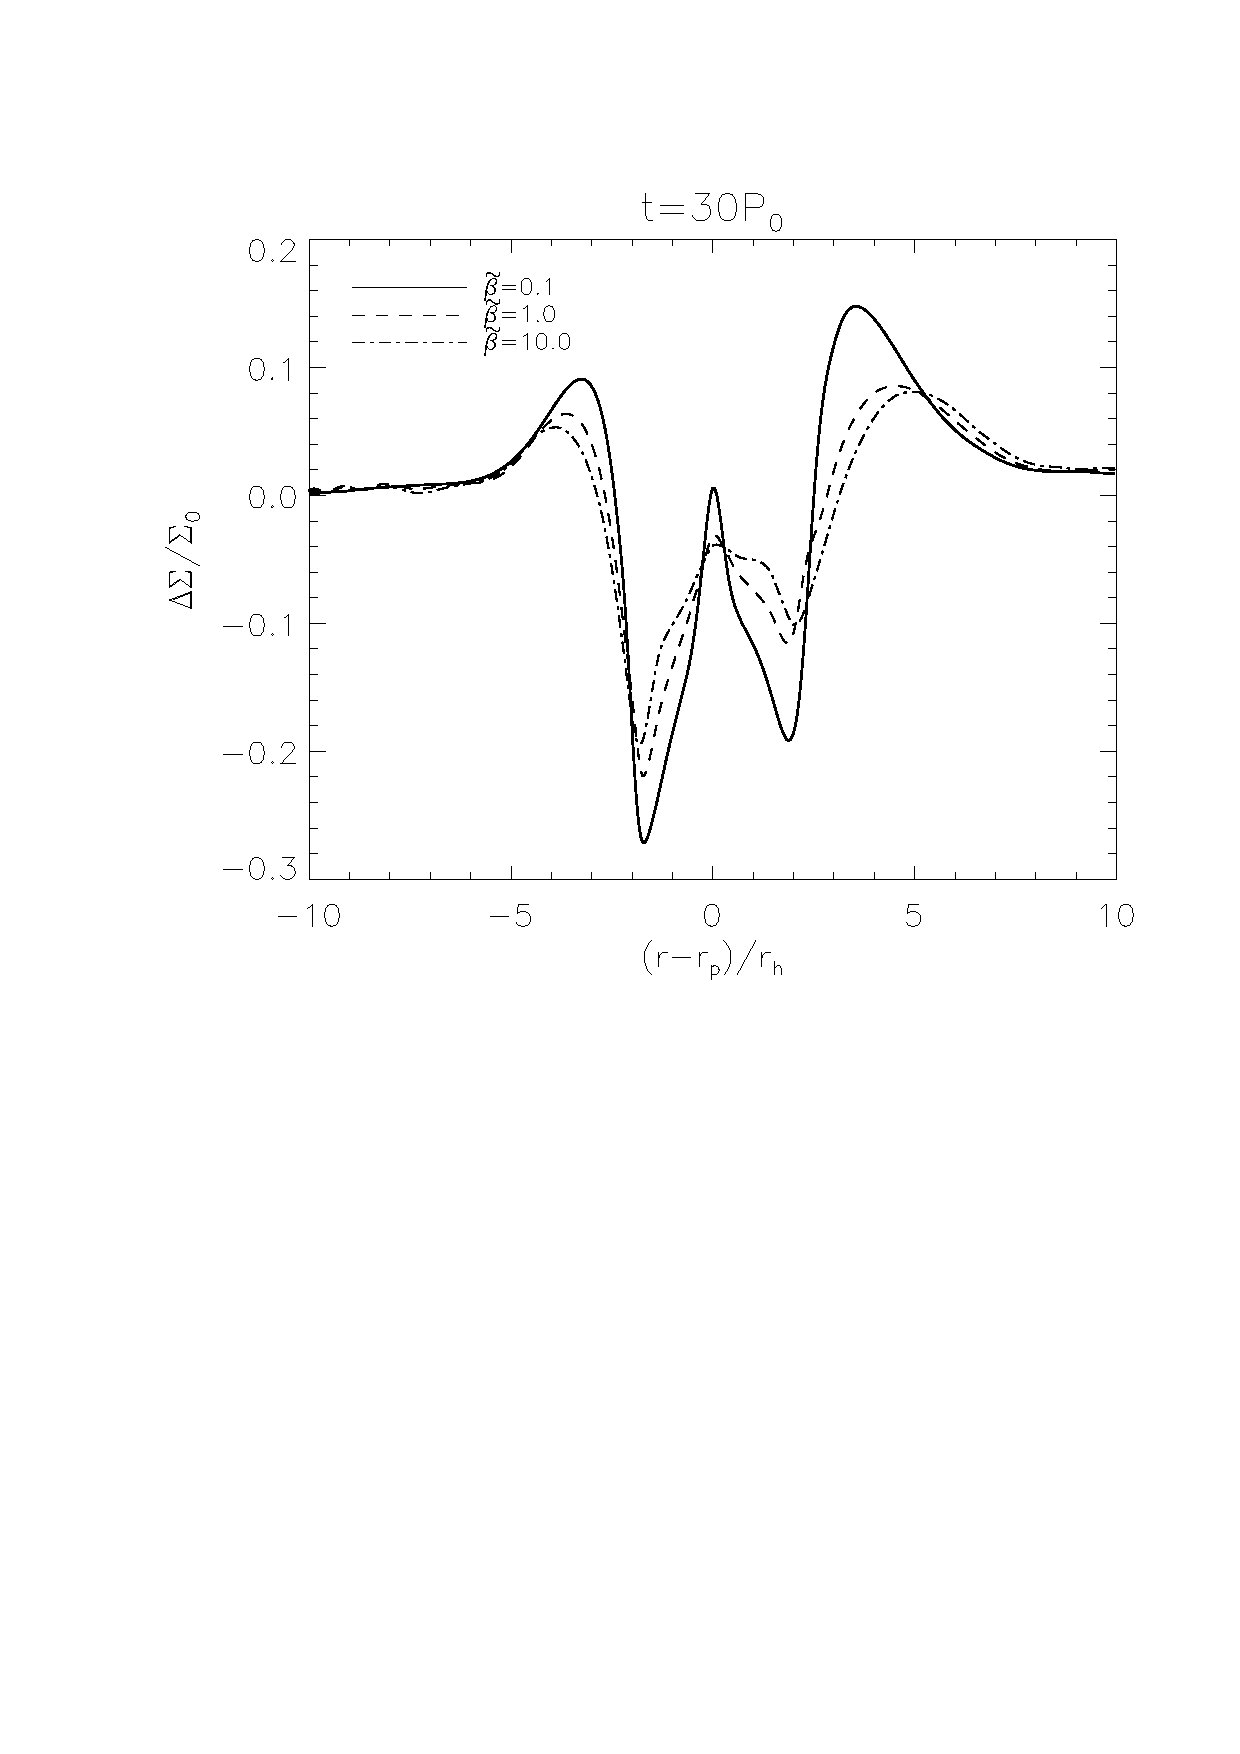
\includegraphics[width=\linewidth,clip=true,trim=0.5cm
    2cm 0cm 0cm]{figures/compare_sigma}
  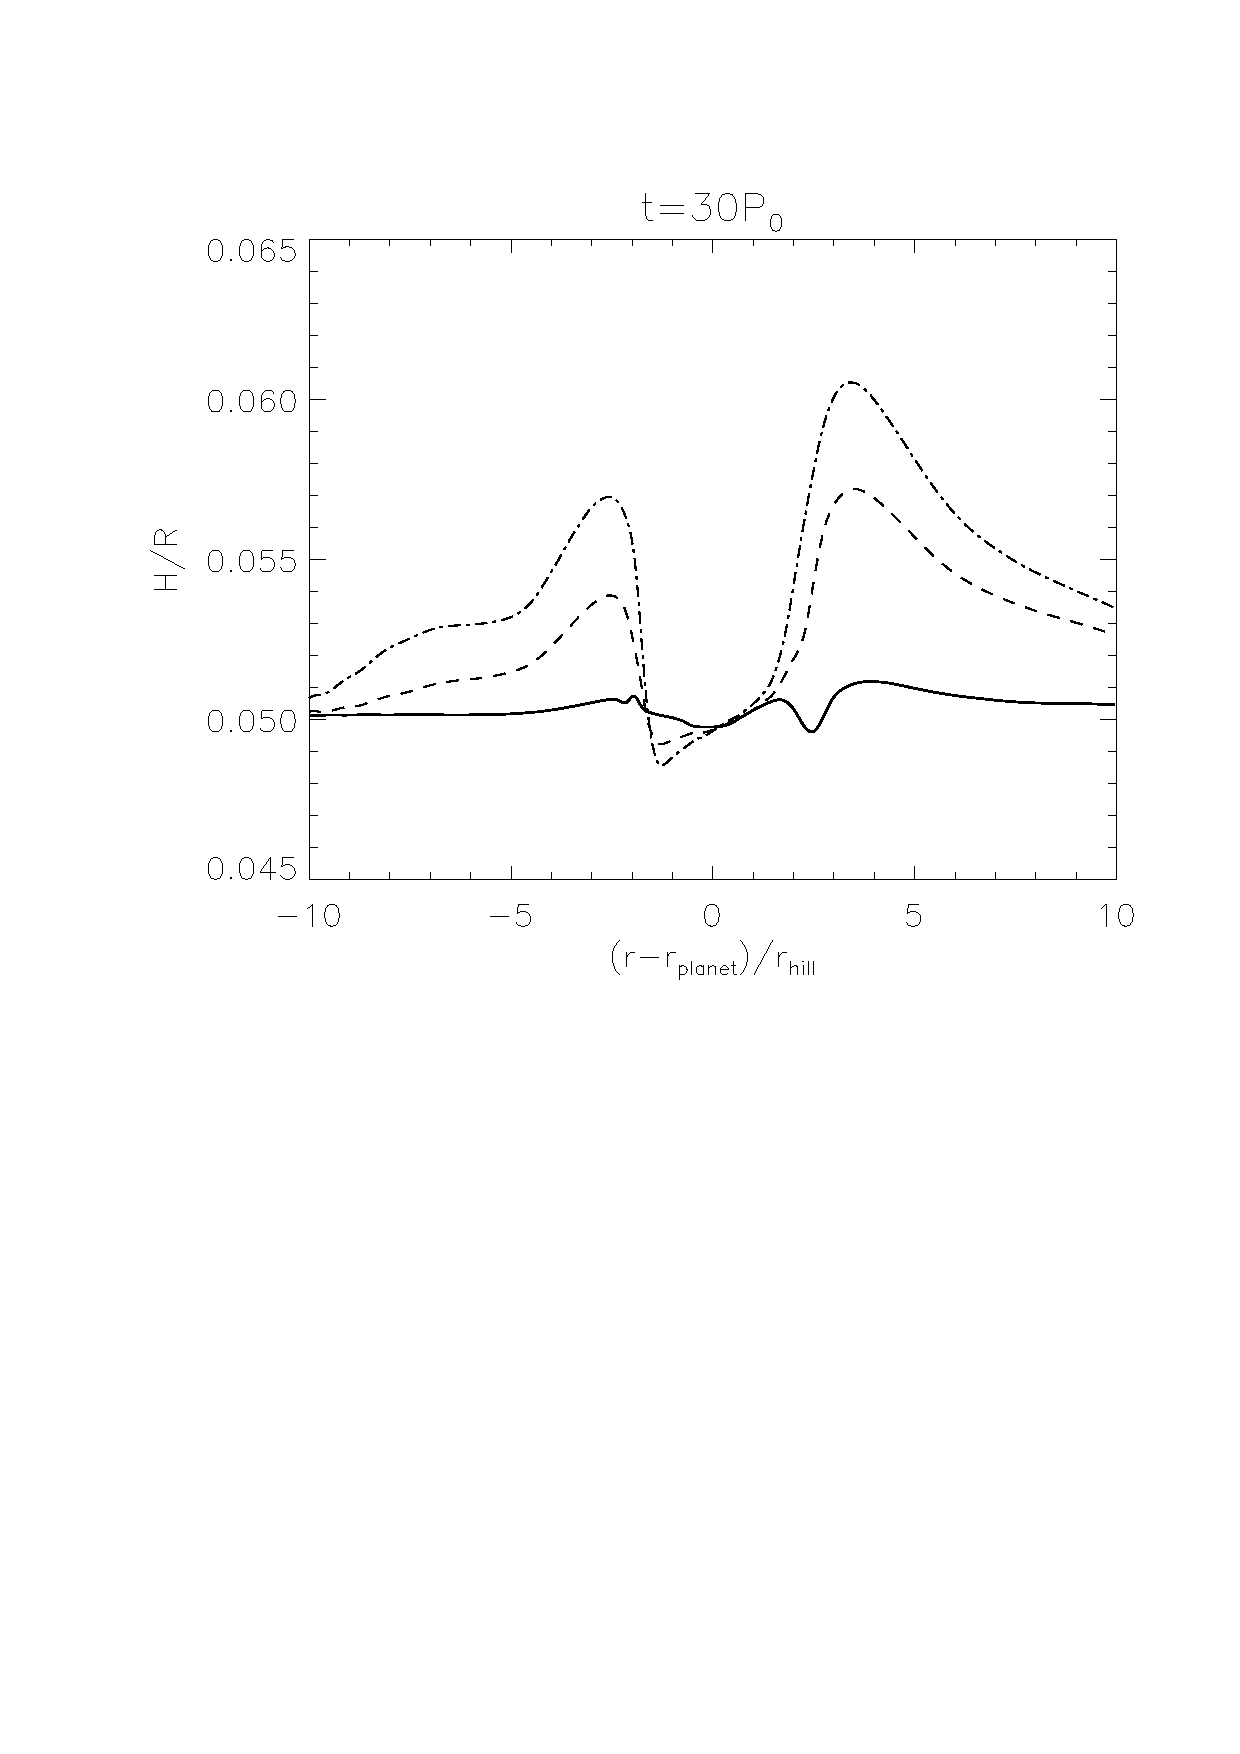
\includegraphics[width=\linewidth,clip=true,trim=0.5cm
    2cm 0cm 1cm]{figures/compare_aspectratio}
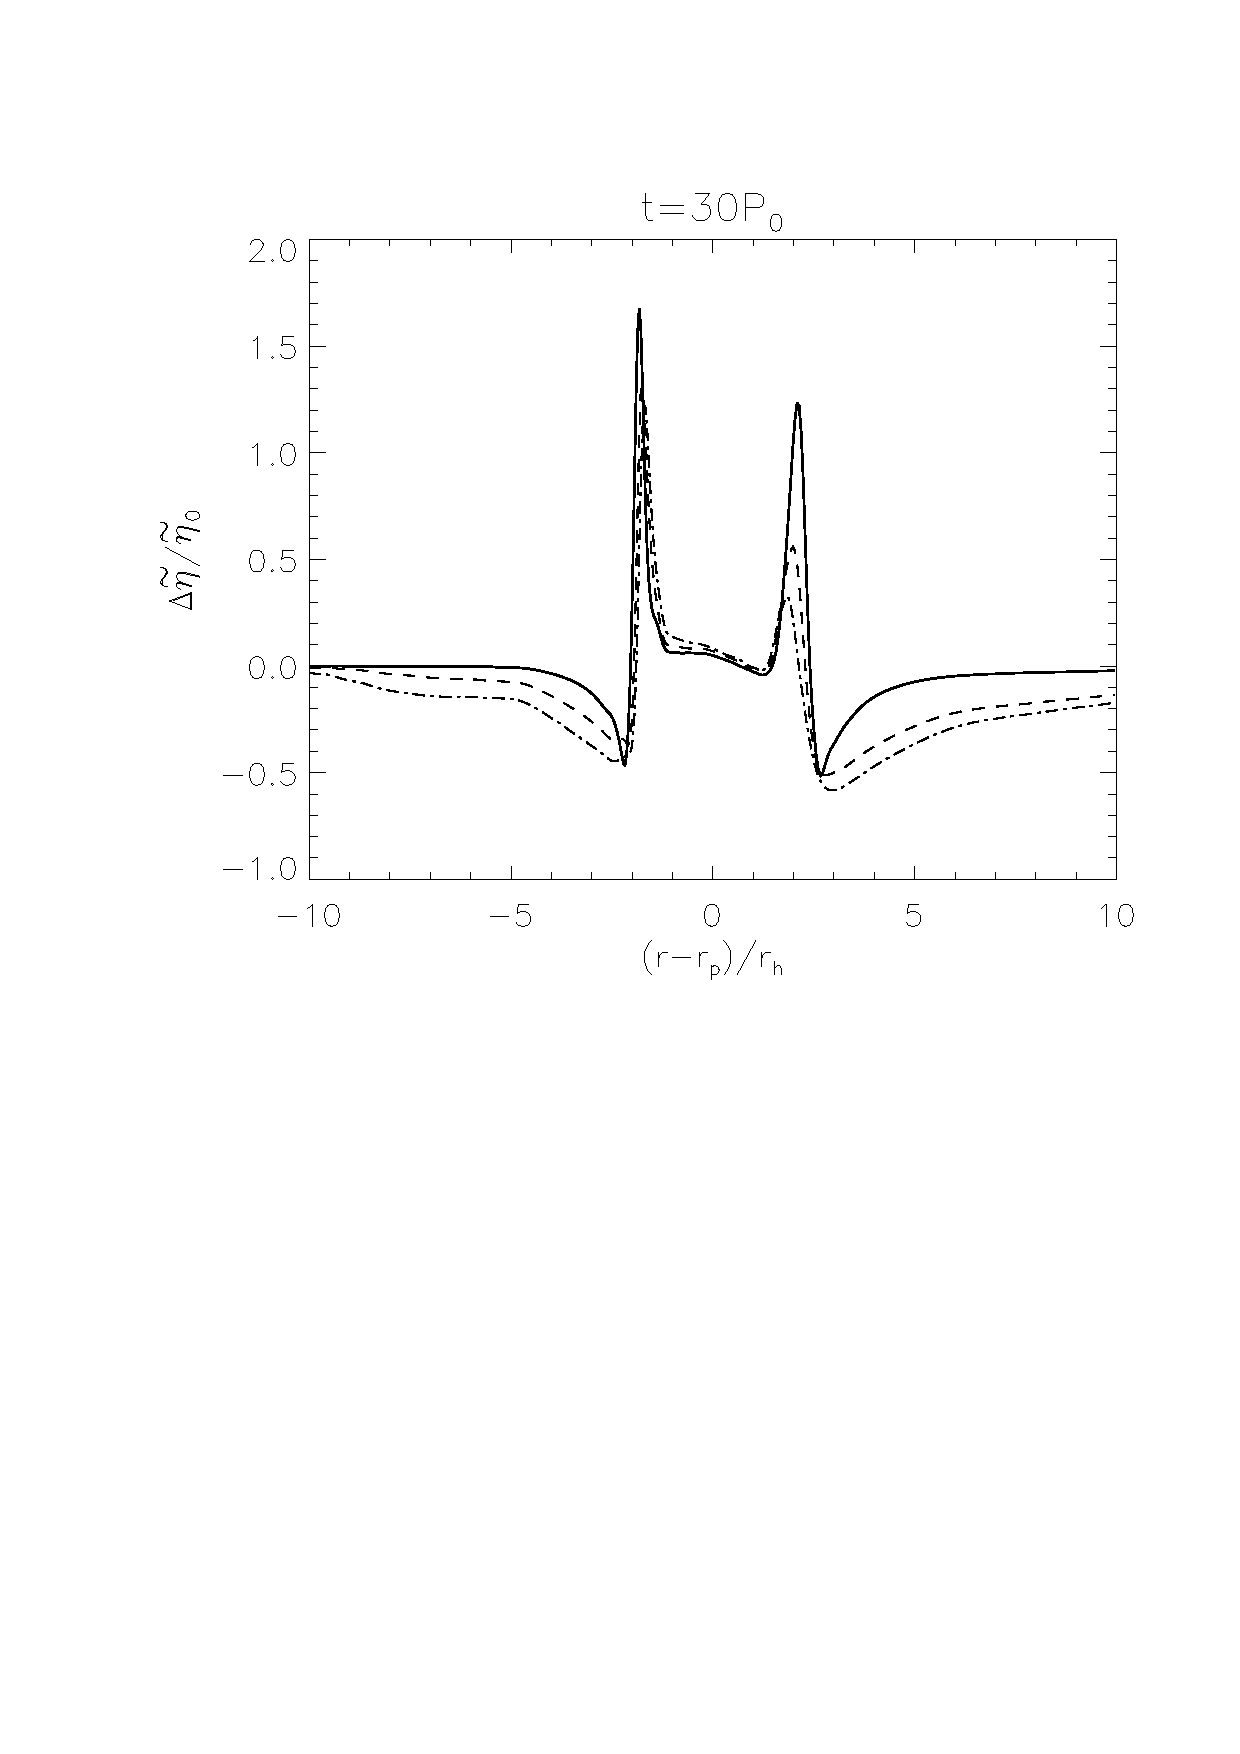
\includegraphics[width=\linewidth,clip=true,trim=0.5cm
    0.5cm 0cm 1cm]{figures/compare_gvortensity}
  \caption{Gap profiles at $t=30P_0$ for the intial partial gap opened
    before instability emerges for fast (solid), moderate
    (dashed), and slow cooling (dashed-dot). The relative surface density
    pertibation (top), disc aspectratio (middle) and generalized
    vortensity pertibation (bottom) are shown. \label{intial1D}}  
\end{figure}


%\begin{tabularx}{0.4\textwidth}{l*{10}{R}} \toprule
%  \multicolumn{11}{c}{$\tilde{\beta}=0.1$} \\ \midrule
%  m                    & 1 & 2 & 3 & 4 & 5 & 6 & 7 & 8 & 9 & 10  \\ 
 % $\gamma10^2/\Omega(r_o)$ & 6.56 & 6.82 & 6.73 & 5.78 & 6.00 & 6.38 & 5.97 & 5.62 & 4.61 & 3.36   \\ \bottomrule
%\end{tabularx}

%\begin{tabularx}{0.4\textwidth}{l*{5}{R}} \toprule
%  \multicolumn{6}{c}{$\tilde{\beta}=1.0$} \\ \midrule
%  m                    & 1 & 2 & 3 & 4 & 5  \\ 
%  $\gamma10^2/\Omega(r_o)$ & 1.27 & 1.28 & 1.35 & 1.01 & 0.61   \\ \bottomrule
%\end{tabularx}

\begin{table}
  \centering
  \caption{Dominant mode and growth rates for
    $\tilde{\beta}=0.1,1.0,10.0$ (fast, moderate, and slow cooling)
    values during `planet-off' simulations \label{modetable}} 
  \hfill
  \begin{minipage}{0.3\linewidth}
    \begin{tabularx}{\textwidth}{l R} 
      \multicolumn{2}{c}{$\tilde{\beta}=0.1$} \\ 
      \toprule
      $m$ & $10^2\gamma/\Omega(r_p)$ \\
      \midrule
      6 & 7.3 \\
      7 & 7.8 \\
      8 & 7.9 \\
      9 & 7.9 \\
      10 & 6.8 \\ 
      \bottomrule
    \end{tabularx}
  \end{minipage}
  \hfill
  \begin{minipage}{0.3\linewidth}
    \begin{tabularx}{\textwidth}{l R} 
      \multicolumn{2}{c}{$\tilde{\beta}=1.0$} \\ 
      \toprule
      $m$ & $10^2\gamma/\Omega(r_p)$ \\
      \midrule
      3 & 2.0 \\
      4 & 2.2 \\
      5 & 2.3 \\
      6 & 1.6 \\
      7 & 1.1 \\ 
      \bottomrule
    \end{tabularx}
  \end{minipage}
  \hfill
  \begin{minipage}{0.3\linewidth}
    \begin{tabularx}{\textwidth}{l R} 
      \multicolumn{2}{c}{$\tilde{\beta}=10.0$} \\ 
      \toprule
      $m$ & $10^2\gamma/\Omega(r_p)$ \\
      \midrule
      1 & 1.1 \\
      2 & 1.6 \\
      3 & 1.7 \\
      4 & 1.2 \\
      5 & 0.1 \\ 
      \bottomrule
    \end{tabularx}
  \end{minipage}
  \hfill
\end{table}

\subsection{Axisymmetric stability}
The intial planet-disc interaction form bumps and grooves in the gap profiles
which can potentially be unstable due to axisymmetric instabilities. The
generalised local axisymmetric stability condition is the Solberg-Hoiland
criterion,  
\begin{align}
  \kappa^2+N^2 \geq 0 
\end{align}
where
\begin{align}
 N^2=\frac{1}{\Sigma} \frac{\partial P}{\partial r}
 \left(\frac{1}{\Sigma} \frac{\partial \Sigma}{\partial
     r}-\frac{1}{\gamma P} \frac{\partial P}{\partial r}  \right) 
\end{align}
is the square of the Brunt-V\"ais\"al\"a frequency. 
At the outer gap edge $r=r_p+2.5r_h$,  where the RWI is excited
(see below), we find $\kappa^2 + N^2$ reaches local minimum with a value
$\sim 0.002$ (code units) for all $\tilde\beta$. The
Brunt-V\"ais\"al\"a frequency is $N\sim 10^{-5}$. 
{\bf Brunt frequency the same for all cooling?}
The Solberg-Hoiland criteria is similary satisfied for the entire disc throughout the 
simulations. {\bf i assume this means the azimuthally averaged
  values. do you ever get $N^2<0$ anywhere in the 2D disc?}  
Thus for all values of $\tilde\beta$ the planet-induced gaps are
stable to axisymmertic instabilities. 

\subsection{Non-axisymmetric instability}\label{linear}
We now examine the evolution of the gap for $t>30P_0$, with the
planet potential switched off, but with an added surface density
perturbation. For all three cooling times $\tilde{\beta}=0.1,\, 1.0,\,
10$, we observe exponential growth of non-axisymmetric
structures.  
An example is shown in Fig. \ref{linearmodes} for 
$\tilde{\beta}=10$. We charcterize these
modes with an azimuthal wavenumber $m$ and growth rate $\gamma(m)$ as defined by
Eq.~\ref{fouriertransform}---\ref{growth}. Mode amplitudes were
averaged over $r-r_p\in[2,5]r_h$. Table \ref{modetable}
lists the growth rates measured during 
linear growth for 5 values of $m$ centred around the maximum. 

\begin{figure}
  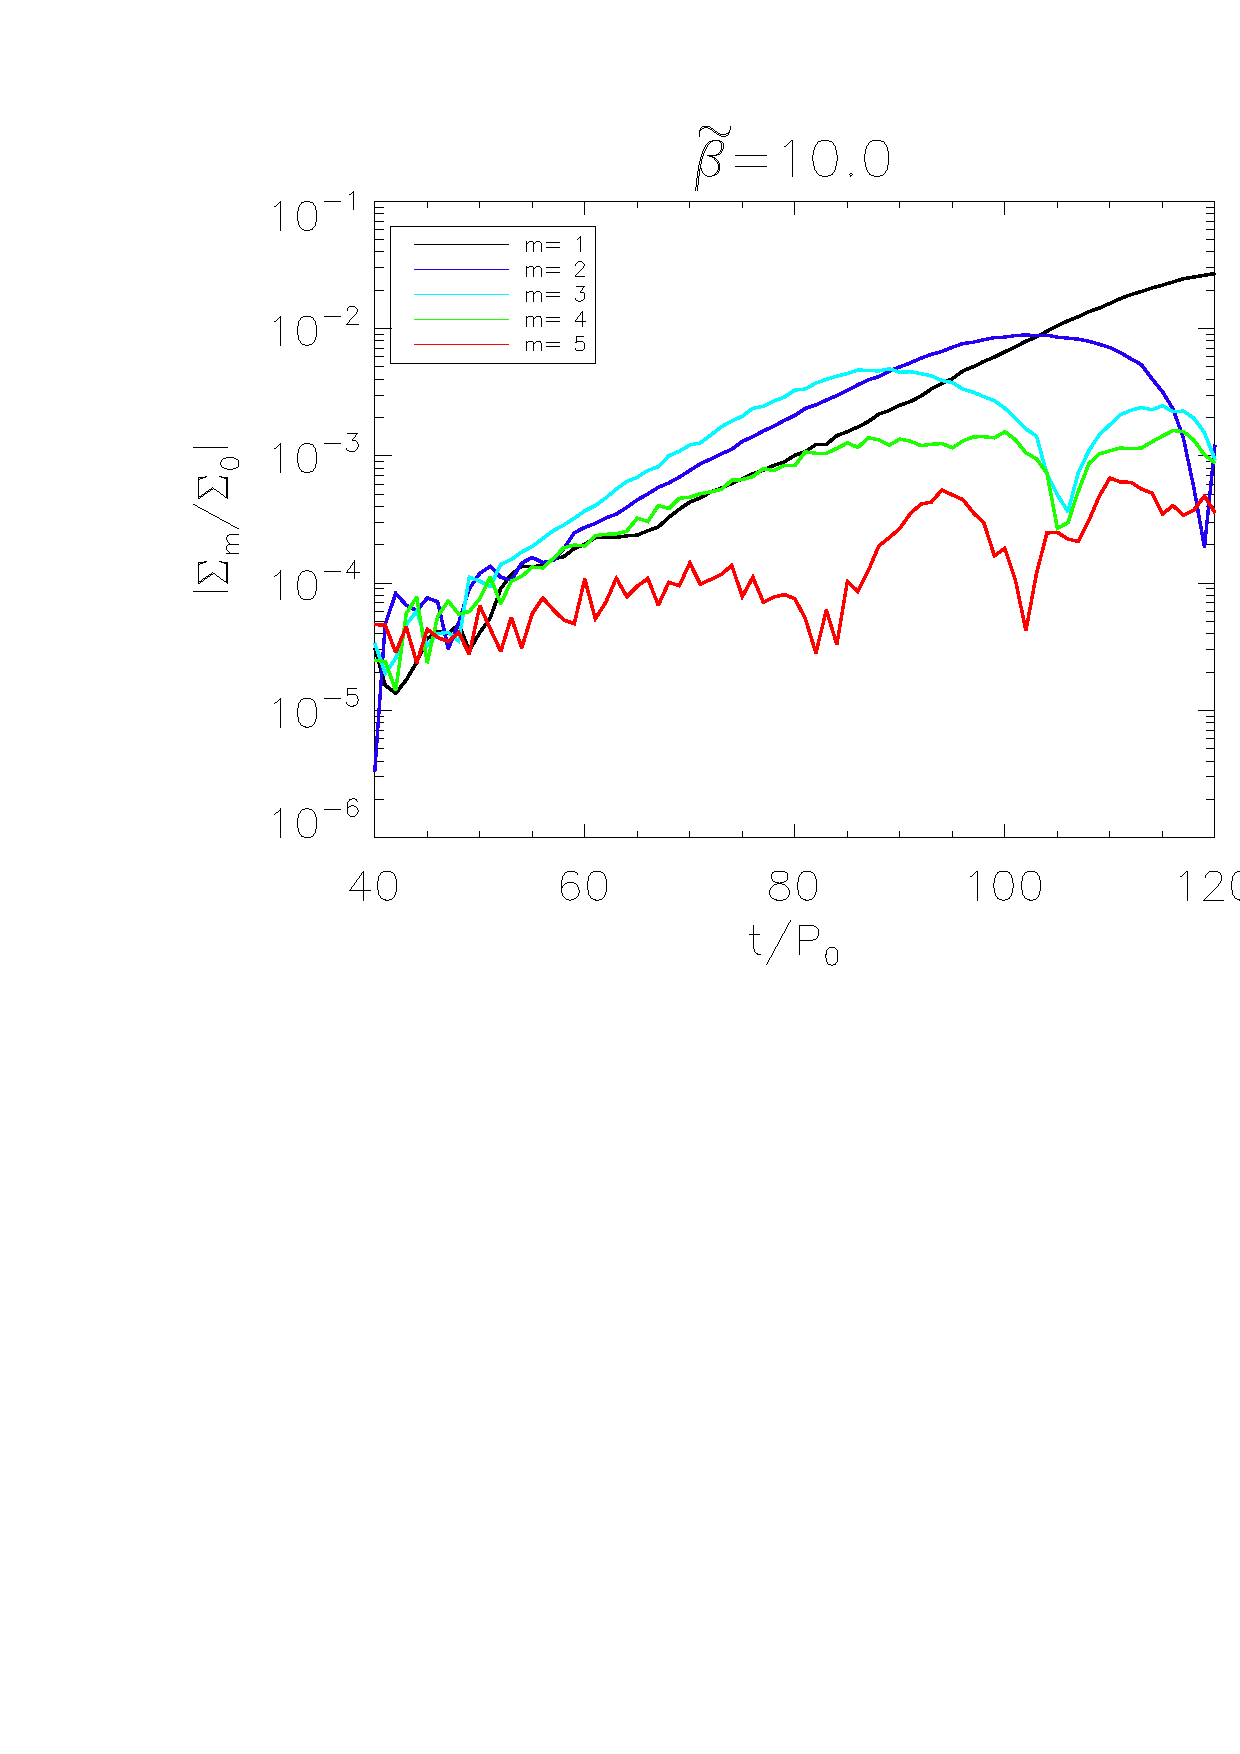
\includegraphics[width=\linewidth,clip=true,trim=1.2cm
  0cm 0cm 0cm]{figures/linear_stability}
  \caption{Evolution of azimuthal Fourier modes of disc surface
    density, non-dimenionlized by the initial axisymmetric background mode 
    $\Sigma_0(t=0)$ for the
    `planet-off' simulations with $\tilde{\beta}=10$. Colours correspond
    to different $m$ values. The $m=3$ component is the fastest growing
    mode during linear growth and has a corresponding
    $\gamma=0.017\Omega(r_p)$.\label{linearmodes}}
  % {\bf is the $\Sigma_0$ at t=0?} }  
\end{figure}

%%%%%%%%%%%%%%%%%%%%%%%%%%%%%%%%%%%%%%%%%%%%%%%%%%%%%%%%%%%%%%%%%%%%%%%

Table \ref{modetable} show that as
$\tilde{\beta}$ is increases from $ 0.1\rightarrow10$ the dominant
azimuthal Fourier mode decreases from $ m=9\rightarrow3$ and the
respective growth rate decreases from $ \gamma/\Omega(r_p)=0.079
\rightarrow 0.017$. However, despite two orders of magnitude increase in the
cooling time, the instability remains dynamical with characteristic  growth time
$\lesssim 10P_0$. Snapshots of the instability in for  
the different $\tilde\beta$ are shown in Fig \ref{2Dlinear}. 

These `planet-off' simulations show that gap edges become more stable with
longer cooling times. This is expected because larger $\tilde{\beta}$
result in hotter gap profiles at $t=30P_0$ with less pronounced
generalized vortensity minima. Stabilization with increased
cooling time is therefore due to a smoother basic state for the
instability, as it is more difficult for the planet to open a gap if
the disc is allowed to heat up. 

\begin{figure}
  \centering
  \subfigure{
    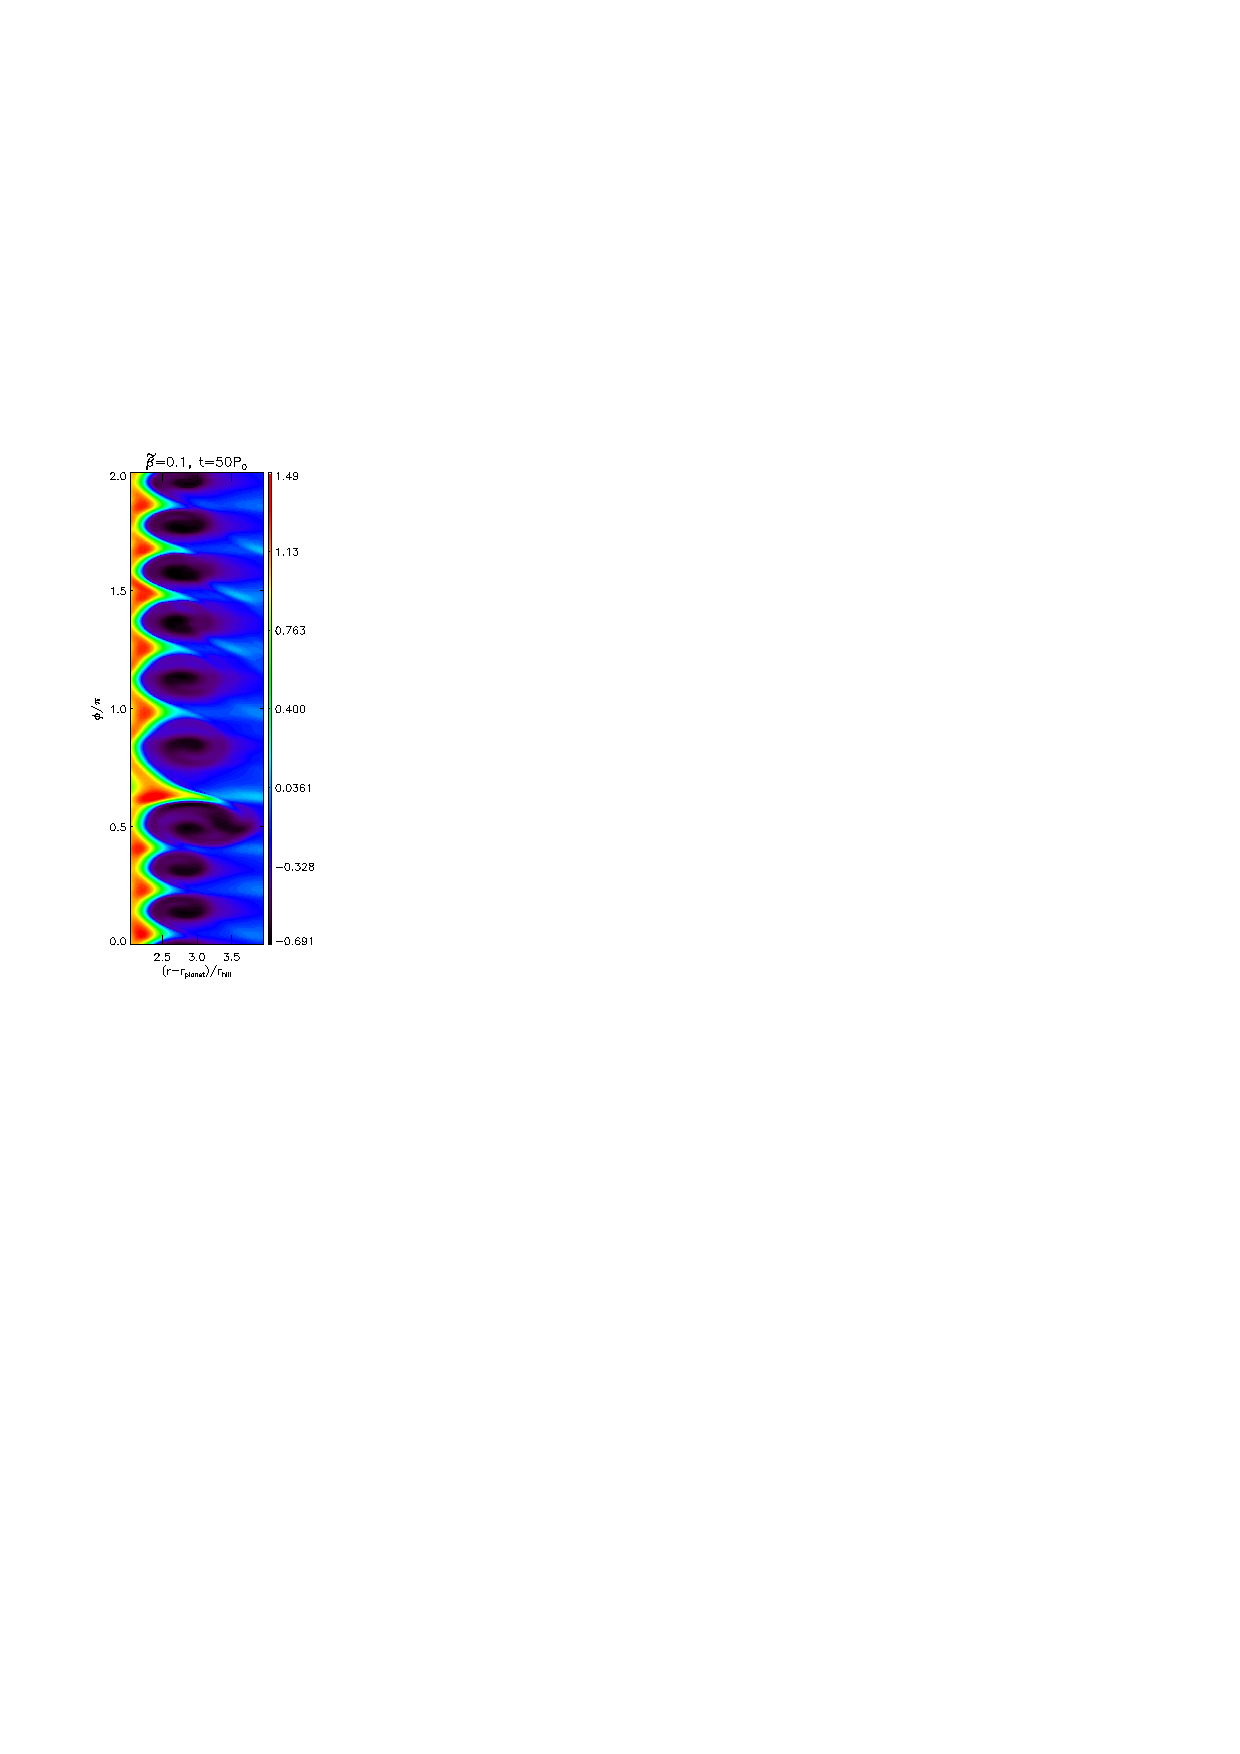
\includegraphics[width=0.3\linewidth]{figures/analysis_gvortensity50}
  }
\hfill
  \subfigure{
    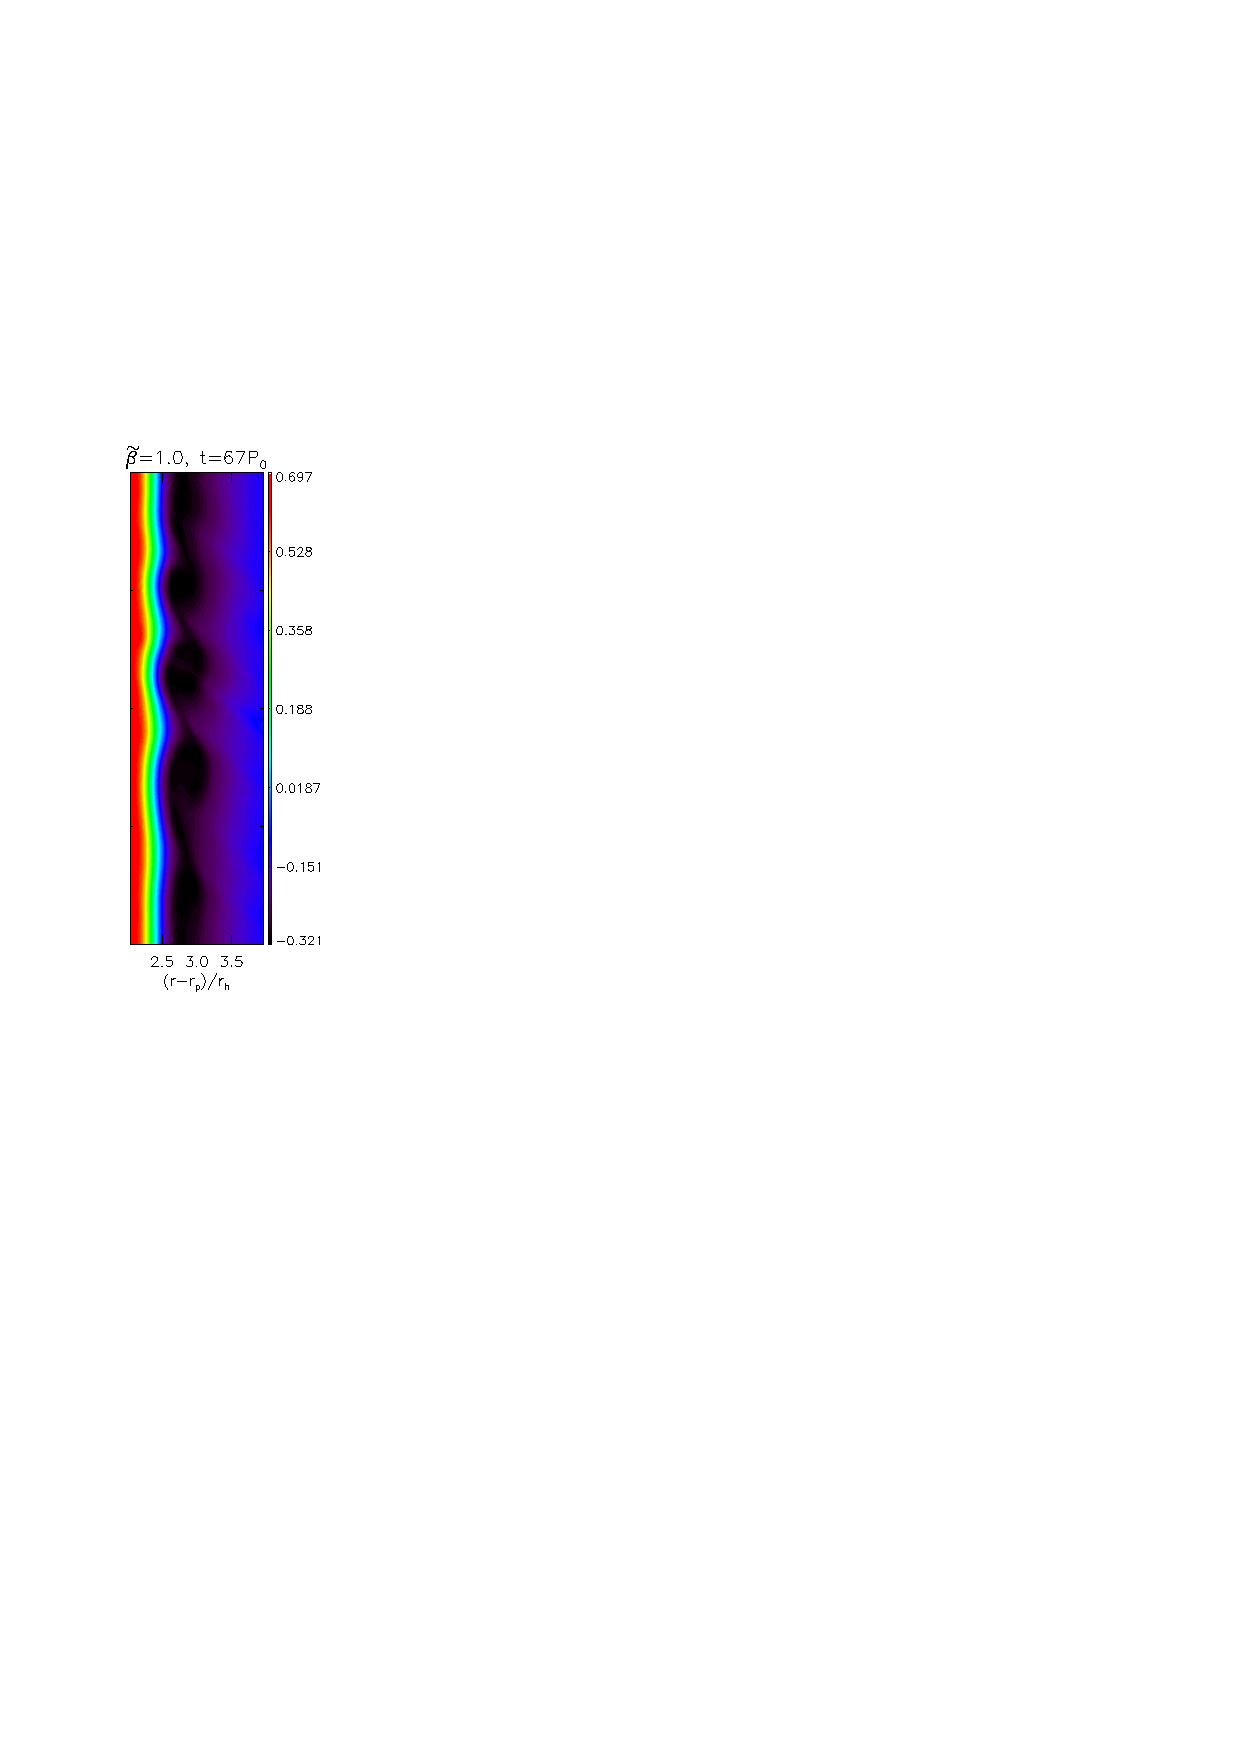
\includegraphics[width=0.3\linewidth]{figures/analysis_gvortensity67}
  }
\hfill
  \subfigure{
    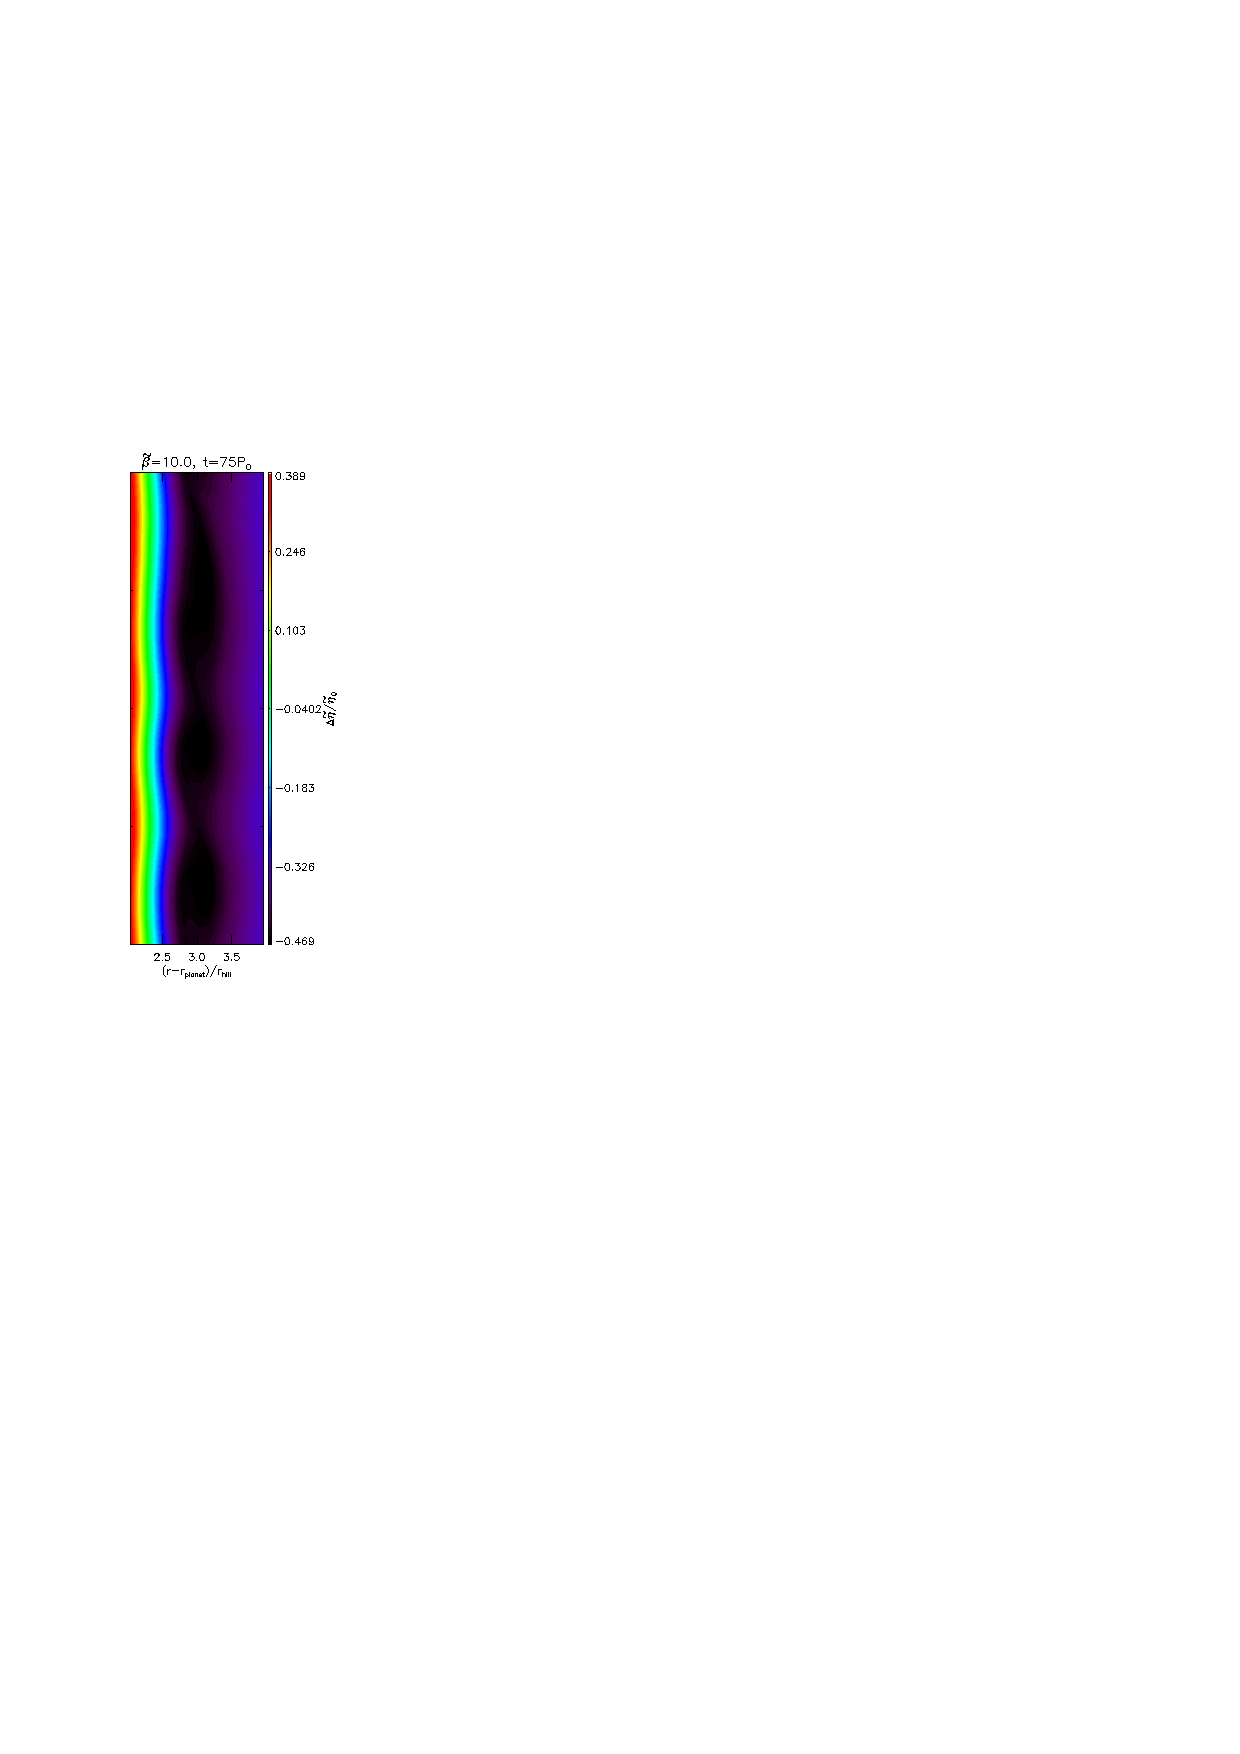
\includegraphics[width=0.3\linewidth]{figures/analysis_gvortensity75}
  }  
  \caption{Generalized vortensity perturbation (relative to $t=0$) for
    cases of $\tilde{\beta}=0.1,1,10$ (left,middle,right) during
    the growth of non-axisymmetric modes. The planet potential has
    been switched off.  The number of vortices
    decrease as $\tilde{\beta}$ increases. Note that snapshots are
    taken later for increasing $\tilde{\beta}$ because it takes longer
    for the vortices to grow and become visible with increasing cooling time. 
    \label{2Dlinear} 
  } 
\end{figure}

\subsubsection{Nearly adiabatic discs}
\label{adiabatic_section}

The above `planet-off' simulations are not formally linear
stability calculations, because the cooling time is shorter
than the instability growth time, 
$t_c<\gamma^{-1}$.  
Thus the disk cools back to its intial temperature corresponding to
$h=0.05$ before or during the instability growth, so we do not
have a steady basic state to formulate a standard linear stability 
problem. 

In order to perform a proper linear stability analysis and capture the
effect of a heated gap edge during instability growth, we ran a simulation  with
$\tilde{\beta}=100$, corresponding to an almost adiabtaic disc.  
In this simulation the cooling rate is slow enough that the gap 
temperature profile (e.g. middle panel of Fig. \ref{intial1D}) changes
only marginally over the instability growth timescale. 

We find very similar gap profiles and mode growth rates for
$\tilde{\beta}=100$ as with $\tilde{\beta}=10$. The disc heats up to
values $h\simeq0.06$ in the nearly adiabatic case. This is close to
the original temperature of $h=0.05$, so linear growth rates are not expected
to change significantly \citep{li00}. 

According to \cite{li00}, increasing $h$ increases linear growth rates
of the RWI because it is pressure-driven. However, in the case 
of disc-planet interaction, increasing $h$ has a stabilizing effect
through the gap profile because it results in smoother gap
edges. The fact that we observe smaller growth rates as $h$ is
increased indicates that for planetary gaps, the importance of $h$ on
the \emph{linear} RWI is through setting up the gap profile, i.e. basic
state for the instability (as opposed to the linear response). 

\subsection{Long term evolution} \label{nonlinearplanetoff} 
{\bf typical rossby numbers for these `planet-off' vortices? do
  stronger vortices (beta=0.1) dissipate faster? if we want to say the
  vortices dissipate viscously, then need to quote a viscosity
  (e.g. reynolds stress) and compute a viscous time and compare to the
  observed decay time. Or attribute to numerical viscosity. It might
  be simplest to just say the vortices decay without the planet. This
  section is mainly used to contrast with planet-on simulations, so
  don't need to go into detail. 
}

We also extended these `planet-off' simulations well into the non-linear
regime. After the linear growth phase of the vortices, vortex merging
takes hold on timescales of up to $150P_0$, until there is one vortex
left. We find the vortex merging
time is depedendent on the growth rates of the modes and saturation
timescales, with the slowest growing modes in $\tilde\beta=10$ taking
the longest to merge.  

Fig.\ref{planetofflifetimeplot} shows evolution of the $m=1$ surface
density amplitude, which represents the post-merger single vortex. For
completeness we also ran intermediate cases with $\tilde{\beta}=0.5$
and $5.0$. The vortices simply decay, on a timescale of $O(10^3)$
orbits. We will see in the next section that this behaviour is very
different to when the planet potential is kept on. Interestingly,
though, vortices arising from the stronger instabilities (shorter
cooling times or lower $\tilde{\beta}$) decays faster.  


\begin{figure}
  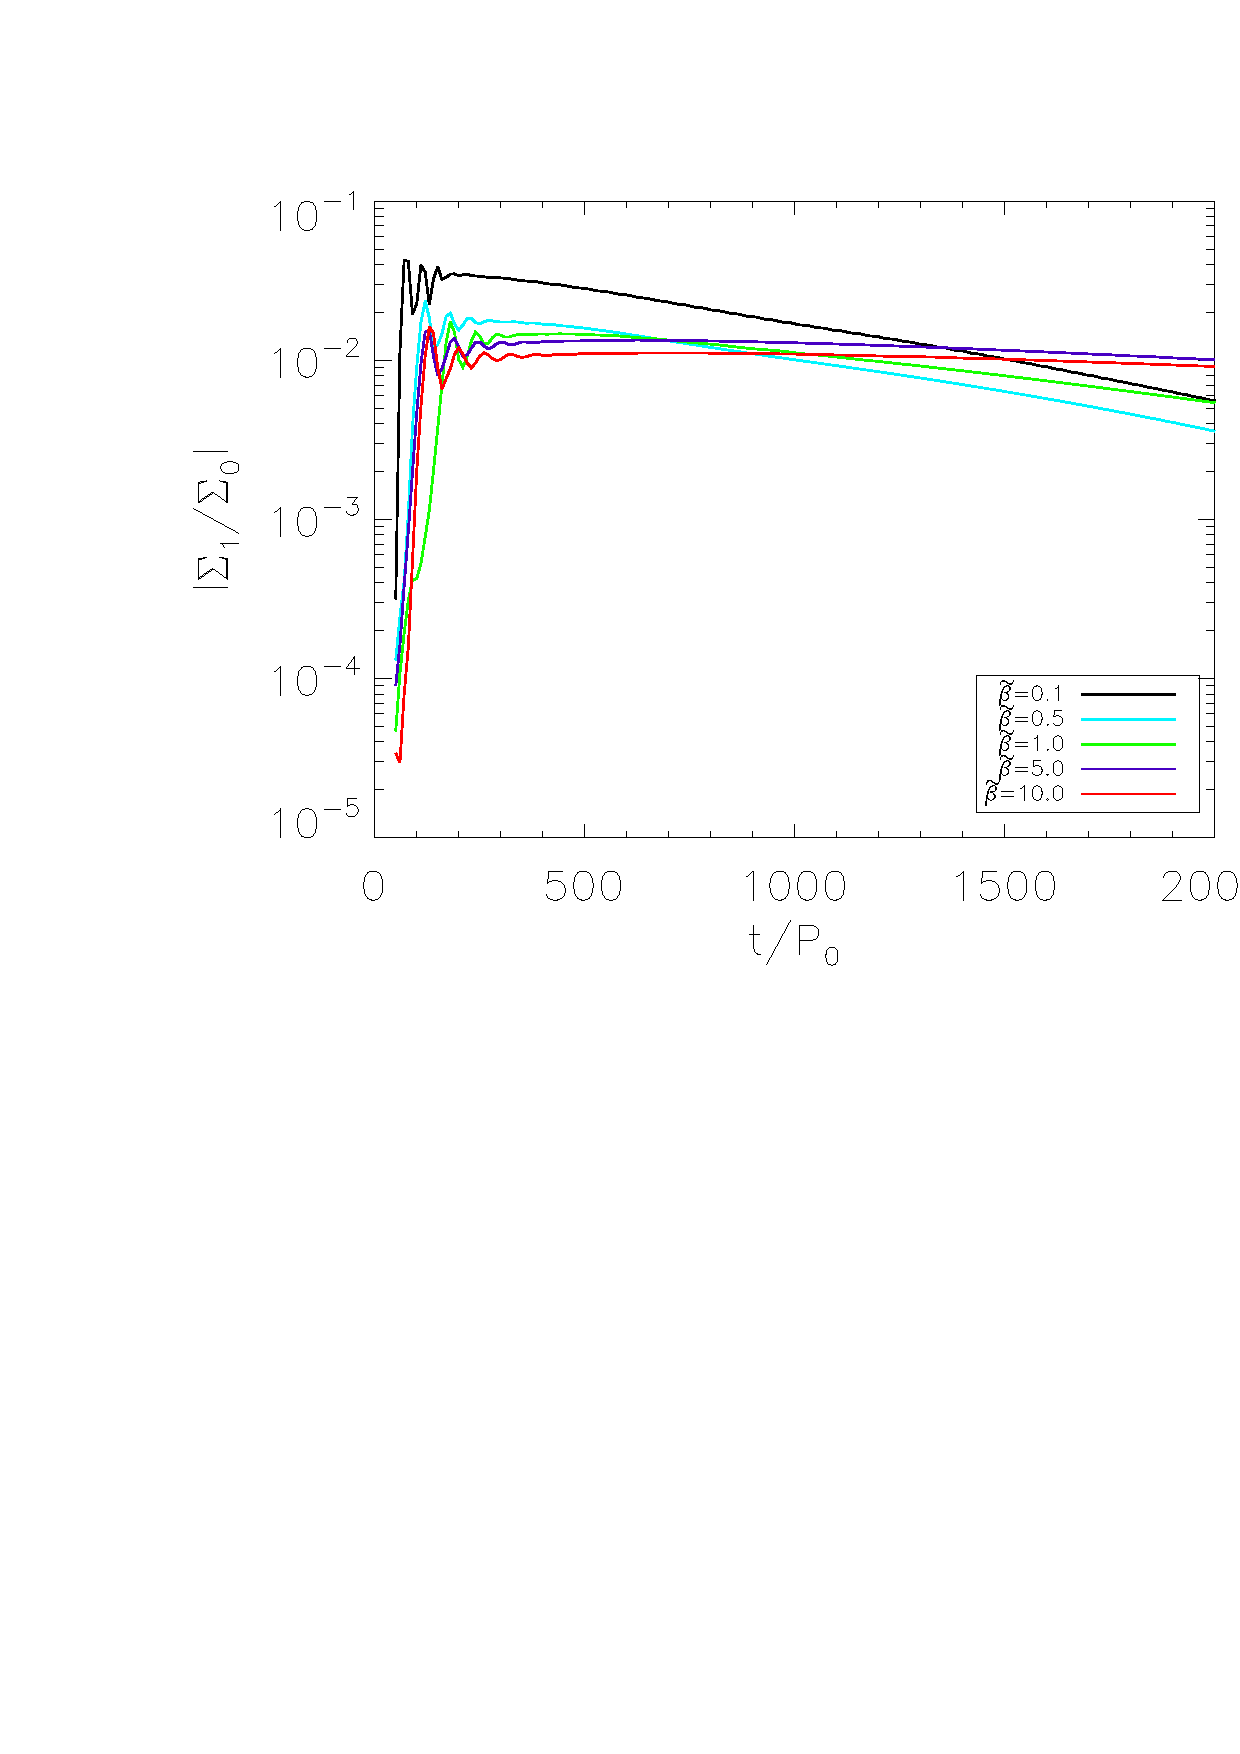
\includegraphics[width=\linewidth,clip=true,trim=0.5cm
  0cm 0cm 1.1cm]{figures/longterm_planetoff}
  \caption{Long term simulations without the planet potential after
    the gap is set up. The $m=1$ surface density component at the
    outer gap edge is shown.
  } \label{planetofflifetimeplot}
\end{figure}

%%%%%%%%%%%%%%%%%%%%%%%%%%%%%%%%%%%%%%%%%%%%%%%%%%%%%%%%%%%%%%%%%%%%%

\section{Non-linear evolution of
  gap-edge vortices with finite cooling time}\label{nonlinear} 
We now examine long-term simulations of gap-edge vortices for
$\tilde{\beta}=0.1,0.5,1,5,10$. The planet potential is kept on
throughout. We employ a grid with $(N_r,N_{\phi})=(512,1024)$ in order
for these 
simulations to be computationally feasible. We also use a larger
disc with $r_{\mathrm{out}}=45r_{\mathrm{in}}$ to minimize boundary
effects on vortex evolution, and apply open boundaries at
$r=r_\mathrm{in},\,r_\mathrm{out}$. We comment that lower-resolution
simulations with $(N_r,N_{\phi})=(256,512)$ were initially carried
out, which show similar behaviour and trends as the high-resolution
runs reported below.   

\subsection{Generic evolution} 
The linear growth of the RWI and vortex-formation is followed by 
vortex merging. We now find merging timescales independent of
$\tilde\beta$, and by $60P_o$ only one vortex remains. 
The evolution of the amplitude of the $m=1$ surface density component,
averaged over $r-r_p\in[2,10]r_h$, is shown in Fig.~\ref{lifetimeplot} 
for different $\tilde\beta$. 
%{\bf any particular reason for the larger radial range for average?
%  did we get bigger vortices?:Yes vortices get quite large in quais steady,
% changing the planet off averaging range to [2,10] changes the plots negligibly
% if we want to just use this value range for consistancy } 

\begin{figure}
  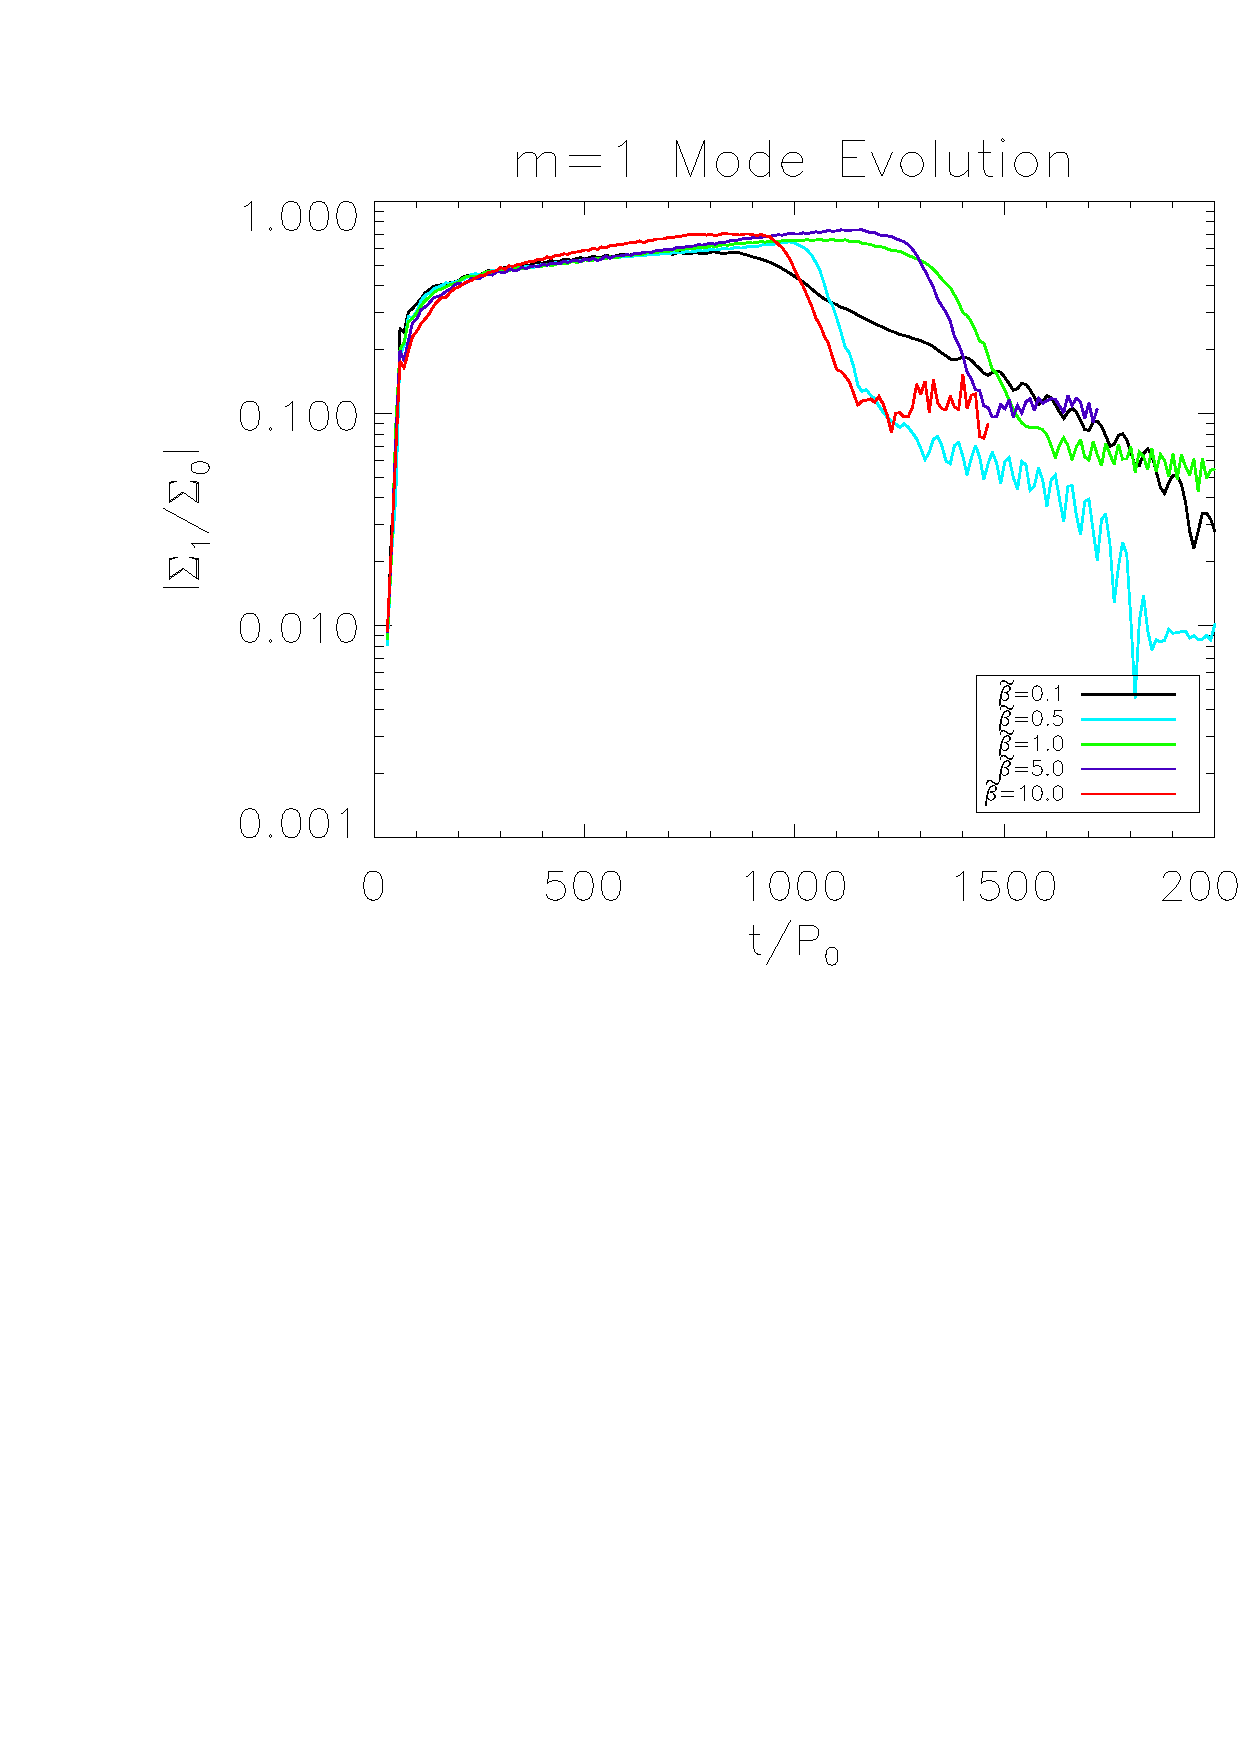
\includegraphics[width=\linewidth,clip=true,trim=0.5cm
  0cm 0cm 1cm]{figures/longterm_stability}
  \caption{Evolution of the $m=1$ surface density component,
    non-dimenionlised by the initial $m=0$ component, for long term
    simulations with the planet potential kept on.\label{lifetimeplot}}   
\end{figure}

In all cases the system remains in a quasi-steady state for
$\gtrsim800P_0$ with a single vortex circulating 
the outer gap edge at the local Keplerian  
frequency. Fig. \ref{Vortex2D} shows a typical plot of the relative 
surface density perturbation in this state. During this stage, the 
vortex intensifies. As the vortex forms it has an initial 
Rossby number $Ro\approx-0.1$ for all $\tilde\beta$
(indicating anti-cyclonic 
motion). As the $m=1$ amplitude grows the Rossby number also increases
in magnitude, 
%relative spin of the vortex
%continuously grows along with it
 reaching a characteristic minimum value of $Ro\approx-0.35$ to $-0.45$ for
all cooling rates. 
{\bf Maybe useful to have a Rossby number v.s. time plot to complement
  mode amplitude plot. 
}
%{\bf is the the value reached just before decay for all cooling?:yes 
%values peak in small range [-0.35,-0.45] for all beta}

We find the vortices can become significantly over-dense. 
The surface density perturbation (relative to $t=0$)  
can reach values of $\Delta\Sigma/\Sigma_0 \sim 7$ at the center of vortices
for all cases of $\tilde\beta$ in quasi-steady state, and
was found as high as $\Delta\Sigma/\Sigma_0 \sim 9$ for the 
$\tilde\beta=10$ case. {\bf any trend between maximum over-density
  achieved and cooling?}
This large increase in surface density is due to  
vortex growth, since there is continuous generation of vorticity by
planet-disc interaction. This is supported by the observation that in
the previous simulations without the planet, the amplitude of
the post-merger vortex does not grow (Fig
\ref{planetofflifetimeplot}).  We remark that the increase in the
vortex surface density directly due to the pile-up of material at the
gap edge (because of gap-opening) is small: the average surface density
perturbation near the outer gap edge, $r\sim r_{p}+2.5r_h$, is 
$\langle\Delta\Sigma/\Sigma_0\rangle_\phi<1$.  

Fig. \ref{lifetimeplot} shows the duration of the quasi-steady state
varies with the cooling rate: for
$\tilde{\beta}=0.1$ and $10$, the vortex amplitude begins to decay around
$t\sim900P_0$, while for $\tilde{\beta}=1,\,5$ the decay begins at 
$t\sim1200P_0$. This non-monotonic dependence suggests that there
exists an optimal cooling rate to maximise the vortex lifetime. We
will discuss this issue futher in
\S\ref{lifetime_discuss}. However, the decay timescale decreases with
increasing cooling time: for $\tilde{\beta}=0.1$ it takes $\sim400P_0$
whereas for $\tilde{\beta}=10$ it takes $\sim 100P_0$ for the $m=1$
amplitude to decay significantly after reaching maximum. 

%These
%timescales are typically much shorter than the duration of the
%quasi-steady state.  

{\bf question: vortex amplitude plot suggest just after linear growth,
  vortex amplitudes are smaller with increasing beta, but later on in
  the quasi-steady state, this trend reverses?  
}
%The
%decay timescale appears to decrease with increasing cooling time. For
%$\tilde{}$  
%Interestingly, in most cases we observe a sudden drop in 
%the $m=1$ amplitude within the simulation time, which occurs over
%timescale between $20P_0$ to $70P_0$, i.e. much shorter than the duration of the
%quasi-steady state. 
%We did not find this dissipation timescale to
%correlate with $\tilde\beta$. 
%We designate the time at which these amplitude drops as the lifetime 
%of the quasi-steady vortex. After the vortices decay the RWI is 
%not seen to be excited again and no vortices are seen to refrom within the
%simulations time. 
{\bf Perhaps a 2D snapshot of what the gap edge looks like after
  vortex death (like the one in the poster). defer definition of
  vortex lifetime to later, when we discuss it. 
}

\begin{figure}
  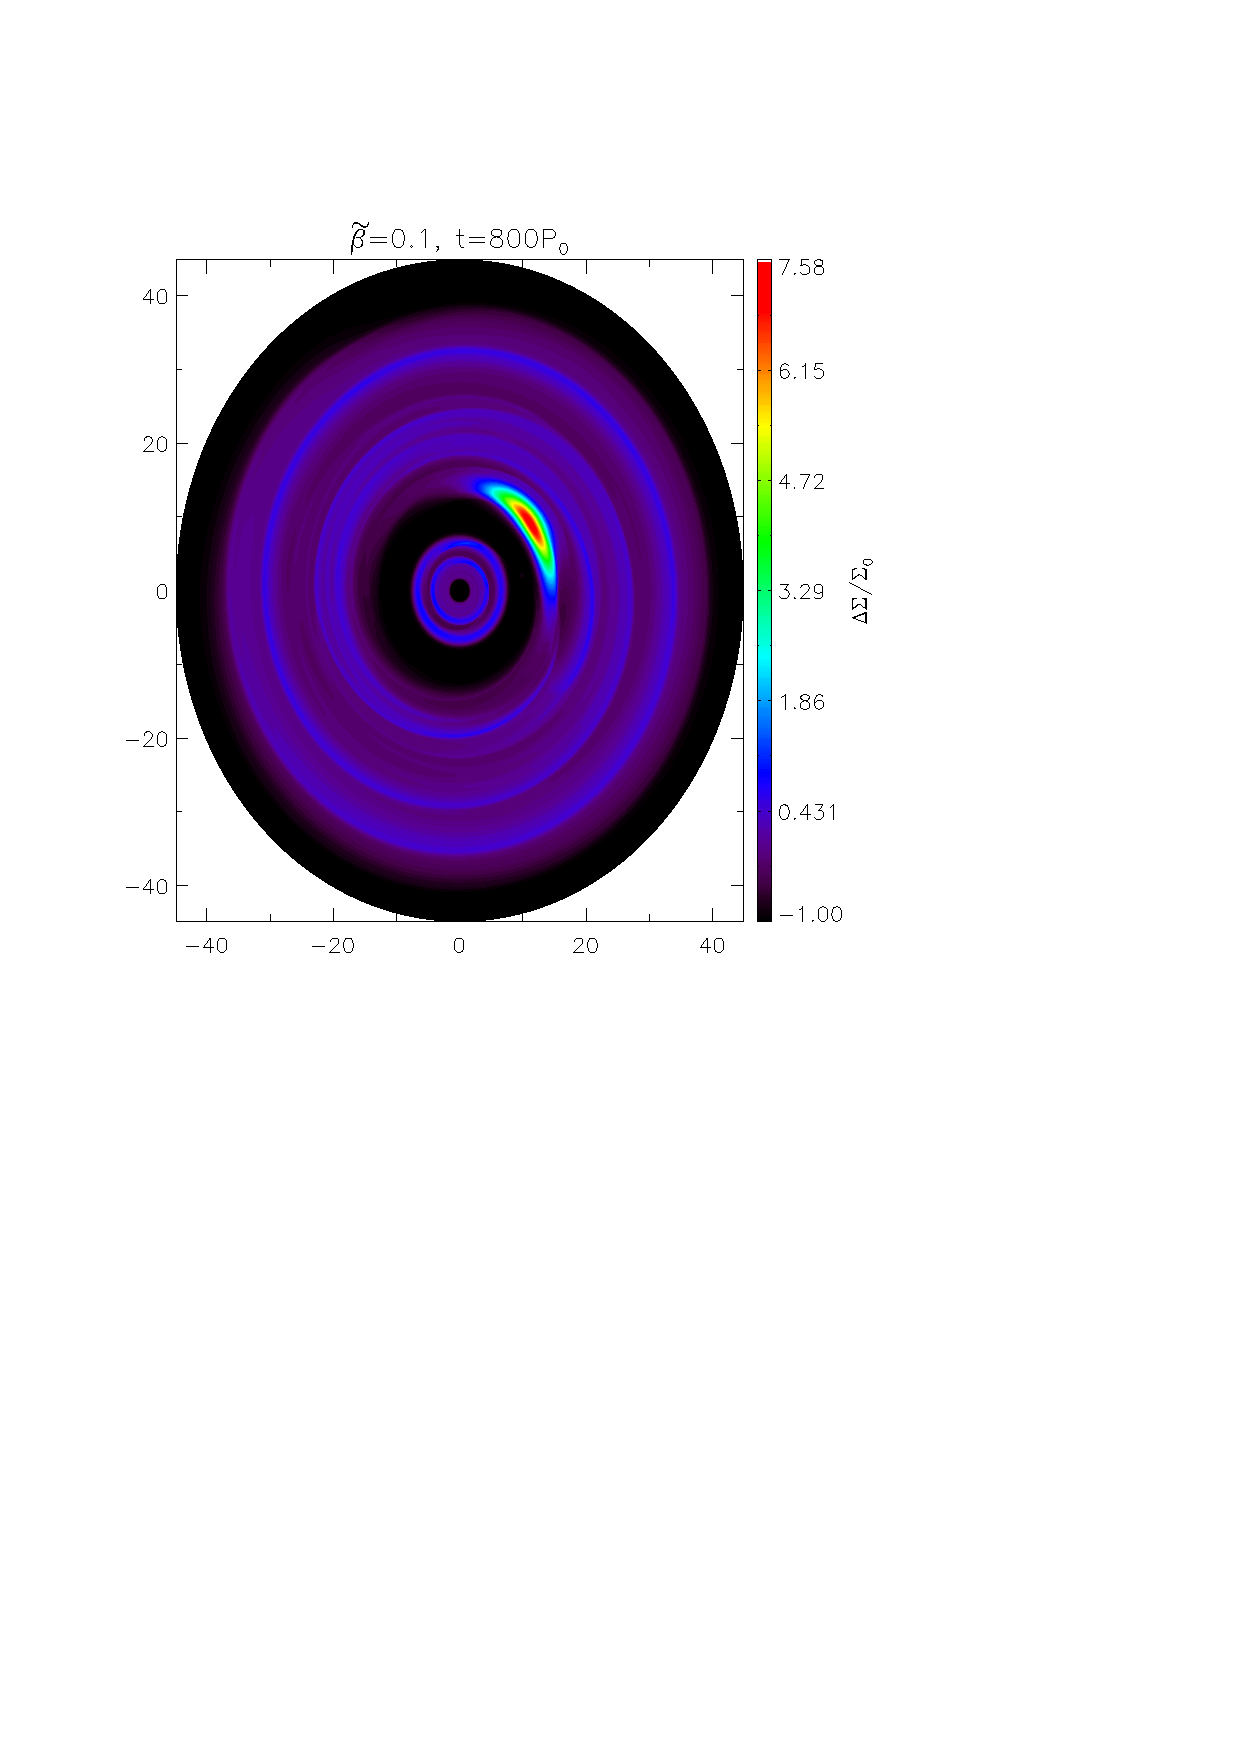
\includegraphics[width=\linewidth,height=\linewidth]{figures/vortex2D}
  \caption{Relative surface density perturbation for the
    $\tilde\beta=0.1$ case during quasi-steady state with a single
    vortex. The plots for other values of the cooling time
    $\tilde{\beta}$ are similar.
    % {\bf is this plot truncated? in the text it says the
    % domain goes to $r=45$?}
    % The large scale non-axisyemetric $m=1$ overdensity can be
    % seen. 
    \label{Vortex2D}} 
\end{figure}

\subsection{Additional analysis on vortex decay}
In this subsection we examine the vortex decay observed in our
simulations in more detail. Fig. \ref{shockplot} show snapshots
of the vortex for the case $\tilde{\beta}=1$. The plots show the surface
density perturbation and the surface density gradient during
quasi-steady state ($t=700P_0$), when the $m=1$ amplitude begins to
decrease ($t=1300P_0$) and just after the rapid amplitude decay
($t=1510P_0$). 

In quasi-steady ($t=700P_0$) the vortex is elongated, but becomes
more compact as it grows before decaying. 
{\bf rough estimate of
  vortex aspect-ratio in the three snapshots? 
  (length/width, by inspection is ok)}  
Notice in Fig. \ref{shockplot} the appearence of wakes extending from
either side of the vortex at $t=1300P_0$. These 
wakes correlate with large gradients in surface density (bottom
panel), and are first seen in the later half of the quasi-steady
state. We find the time at which 
the vortex begins to decay coincides with the emergence of these
wakes. {\bf true statement?}  

% As the vortices grow in intensity wakes are seen to extend from them. 
During quasi-steady state the average value of the surface density gradient
along the wakes is $|\nabla\Sigma/\Sigma| \sim 4 $.{\bf quote something
  dimensionless, or say `in code units'}  
Just before the $m=1$ amplitude begins to decrease, we observe this quantity
sharply increases to $ \sim 6 $, and remains around this value
until the vortex dies out, at which point the associated Rossby number
quickly approaches zero.   

\begin{figure}
  \subfigure{
    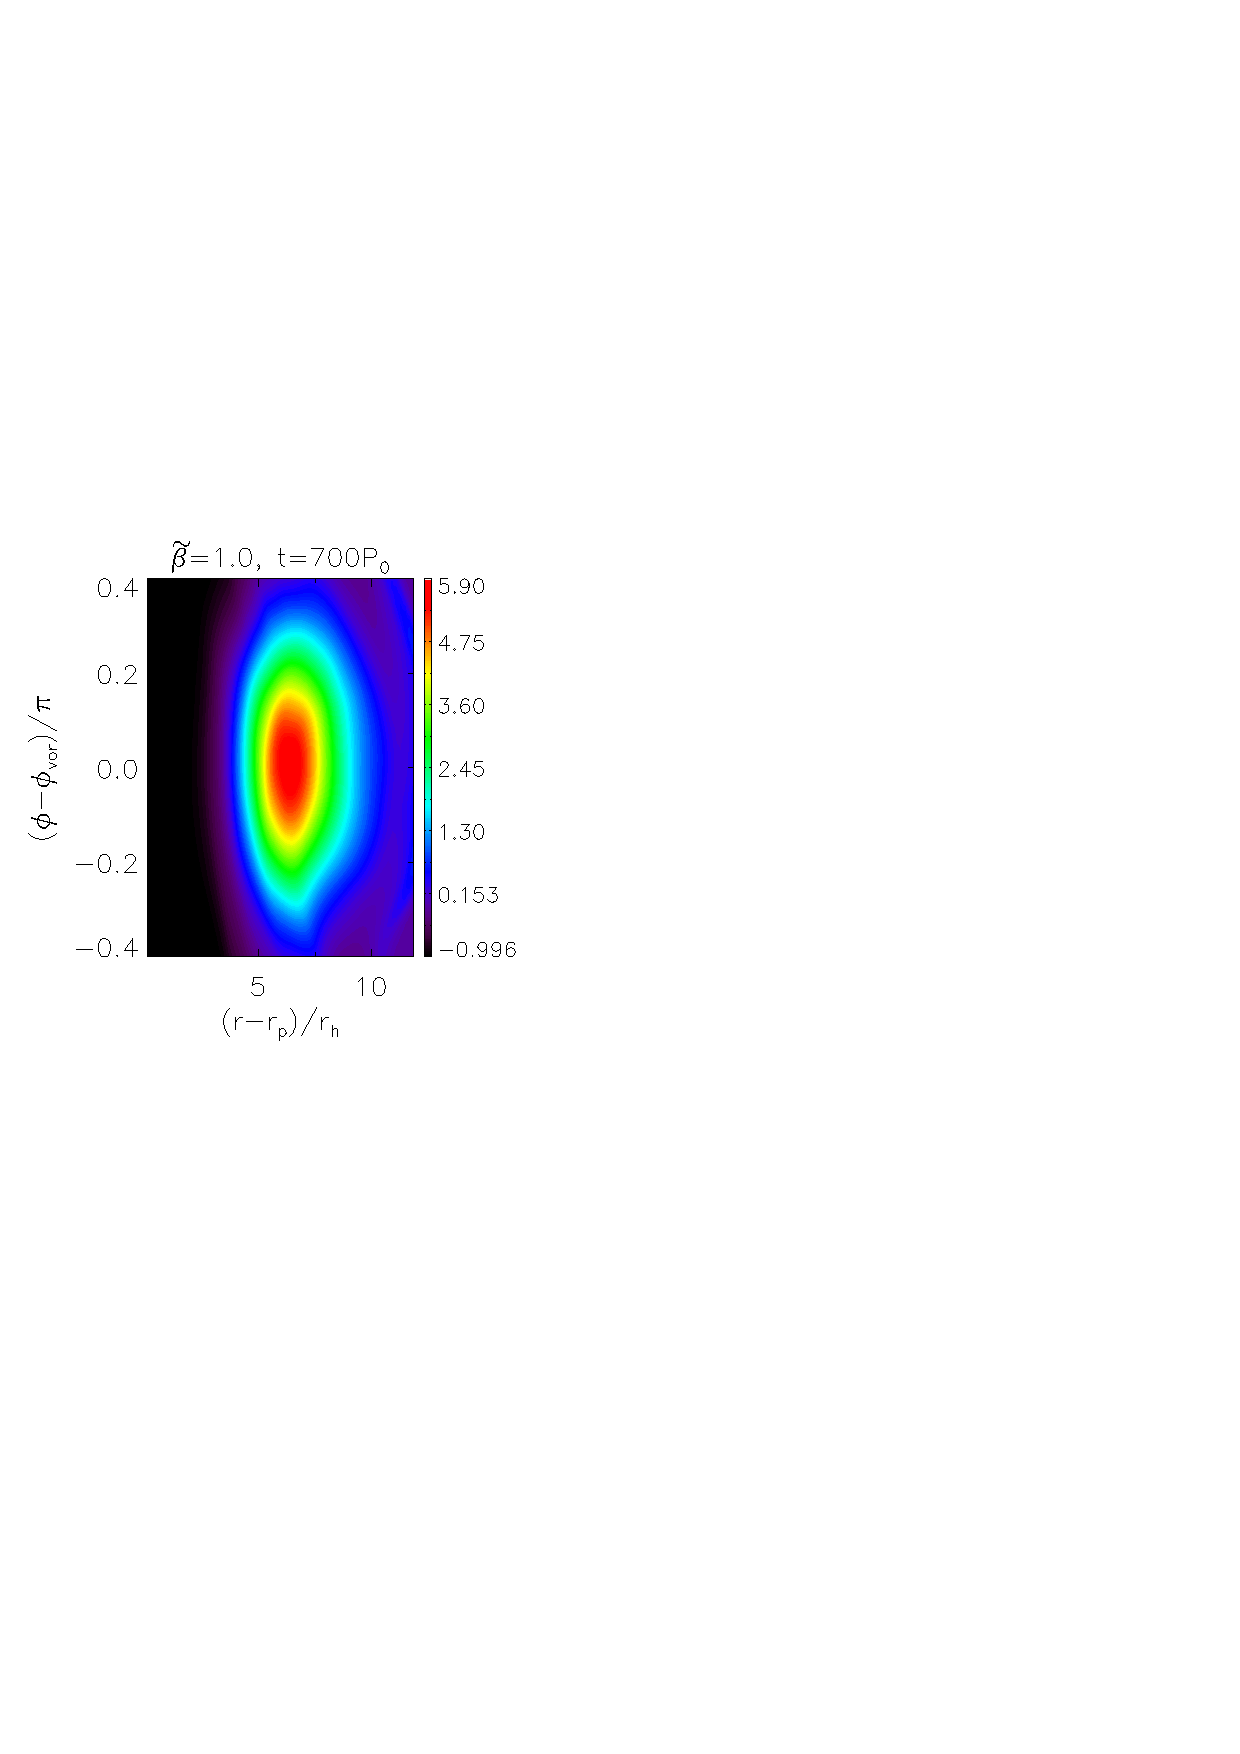
\includegraphics[width=0.3\linewidth]{figures/shock1}
  }
  \hfill
  \subfigure{
    \includegraphics[width=0.3\linewidth]{figures/shock2}
  }
  \hfill
  \subfigure{
    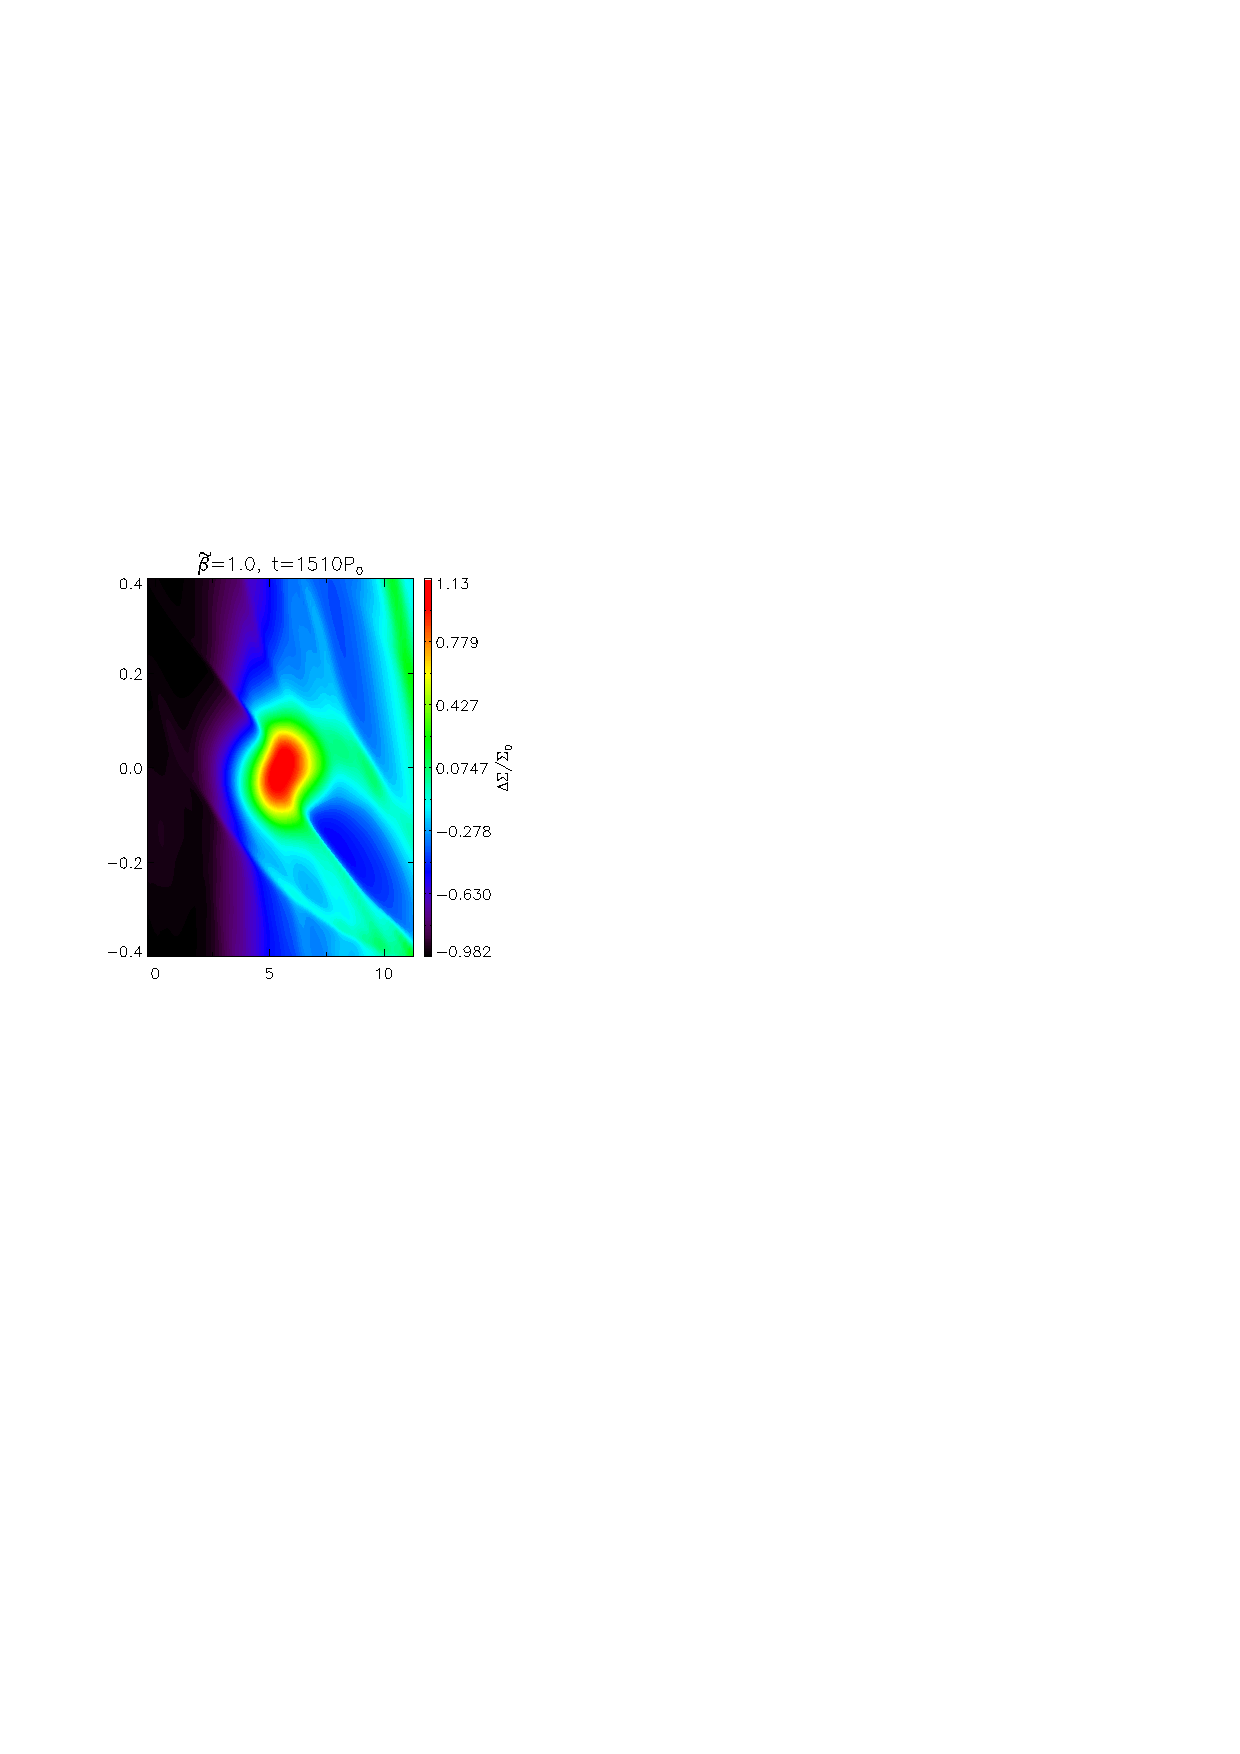
\includegraphics[width=0.3\linewidth]{figures/shock3}
  } \\[-0.98cm]
  \subfigure{
    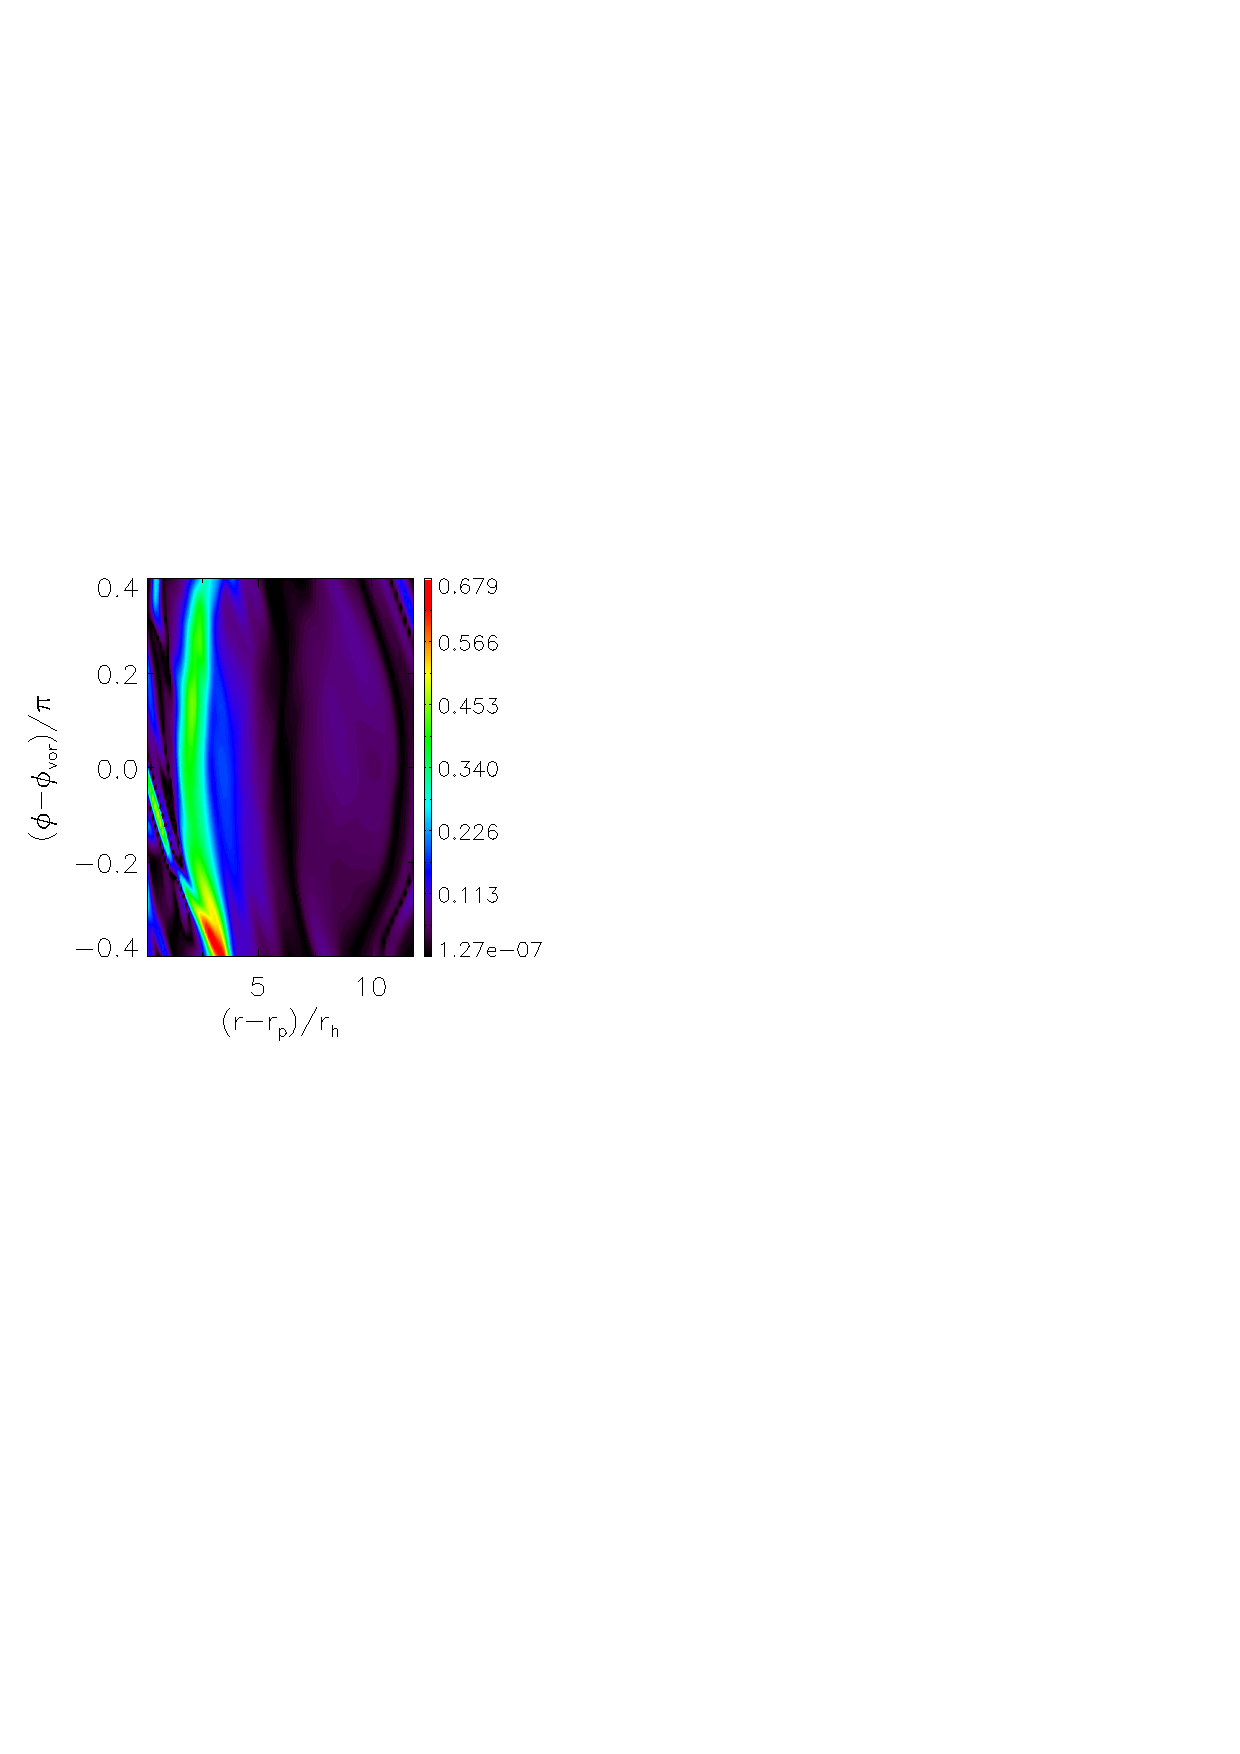
\includegraphics[width=0.3\linewidth]{figures/shock4}
  }
  \hfill
  \subfigure{
    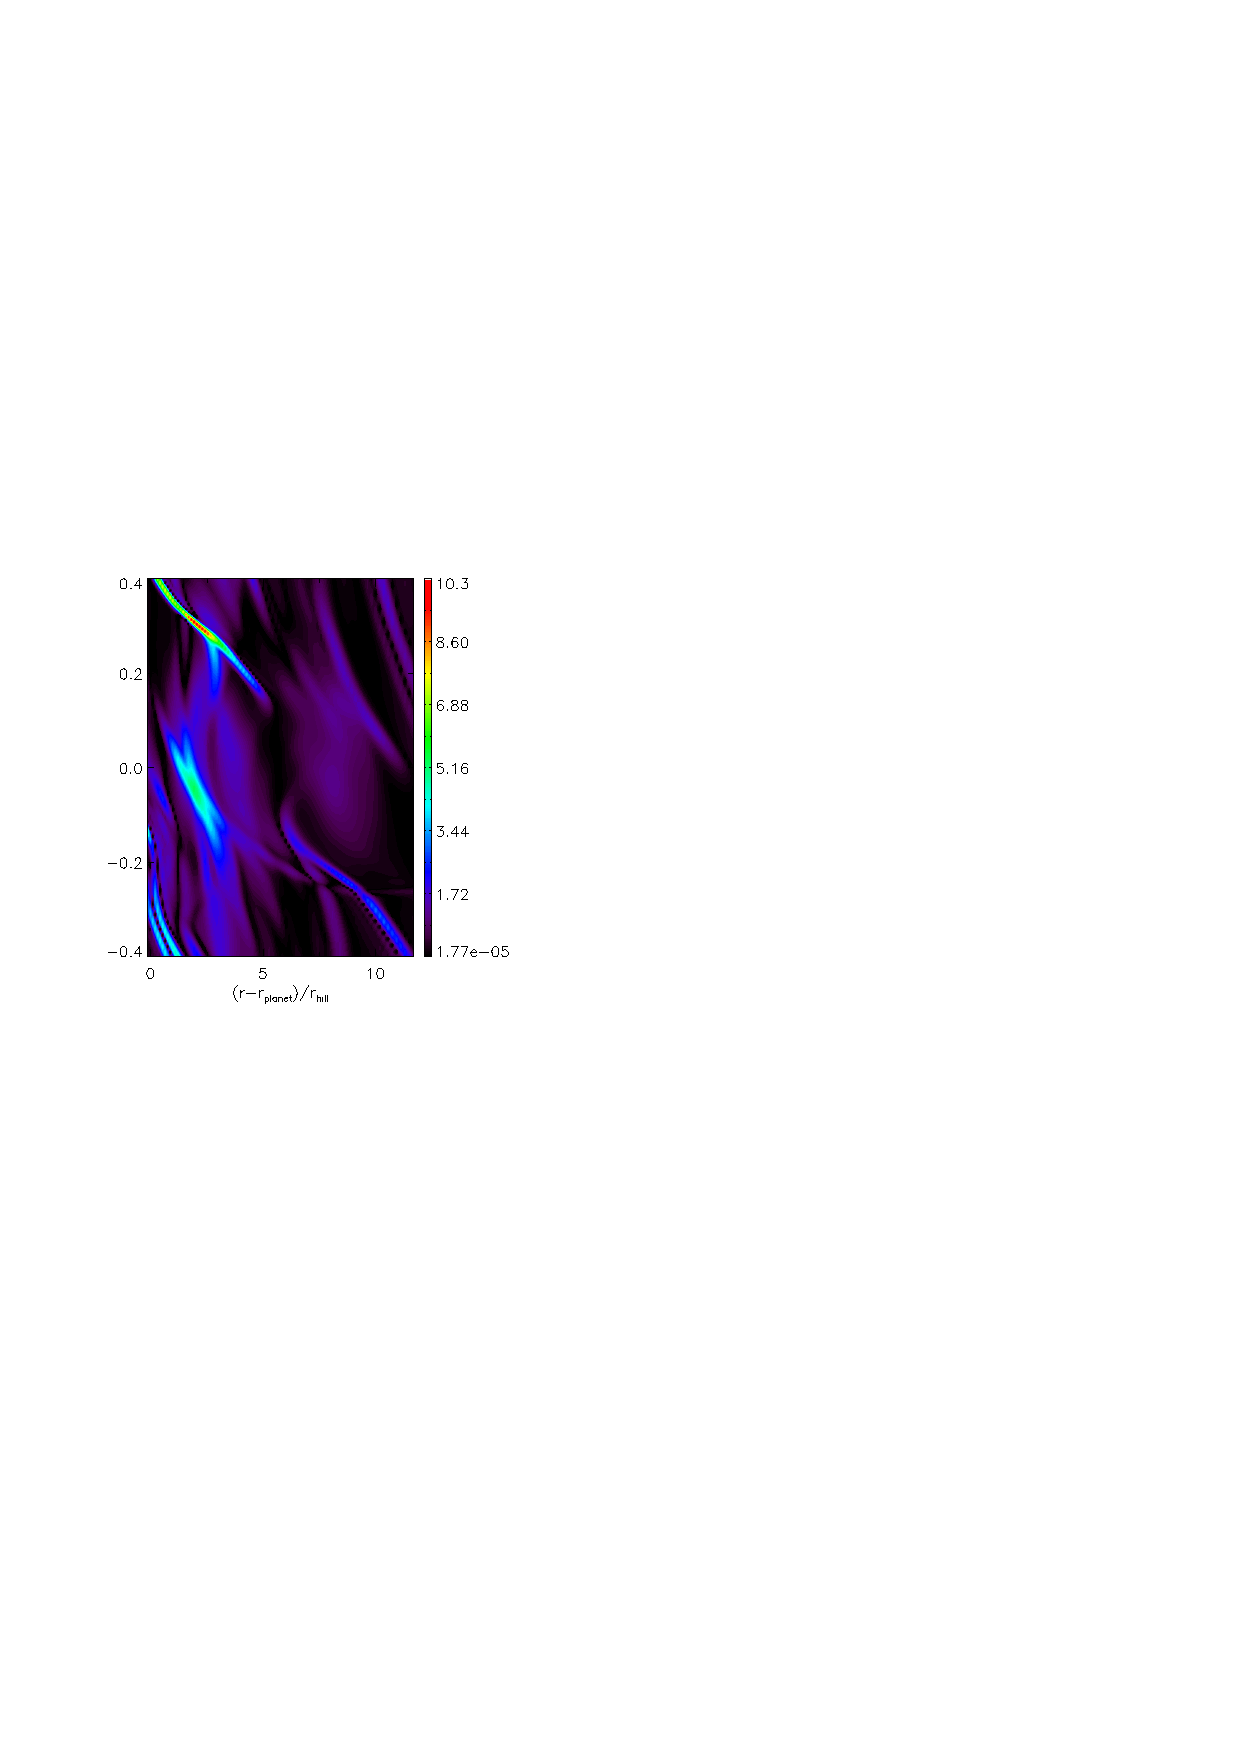
\includegraphics[width=0.3\linewidth]{figures/shock5}
  }
  \hfill
  \subfigure{
    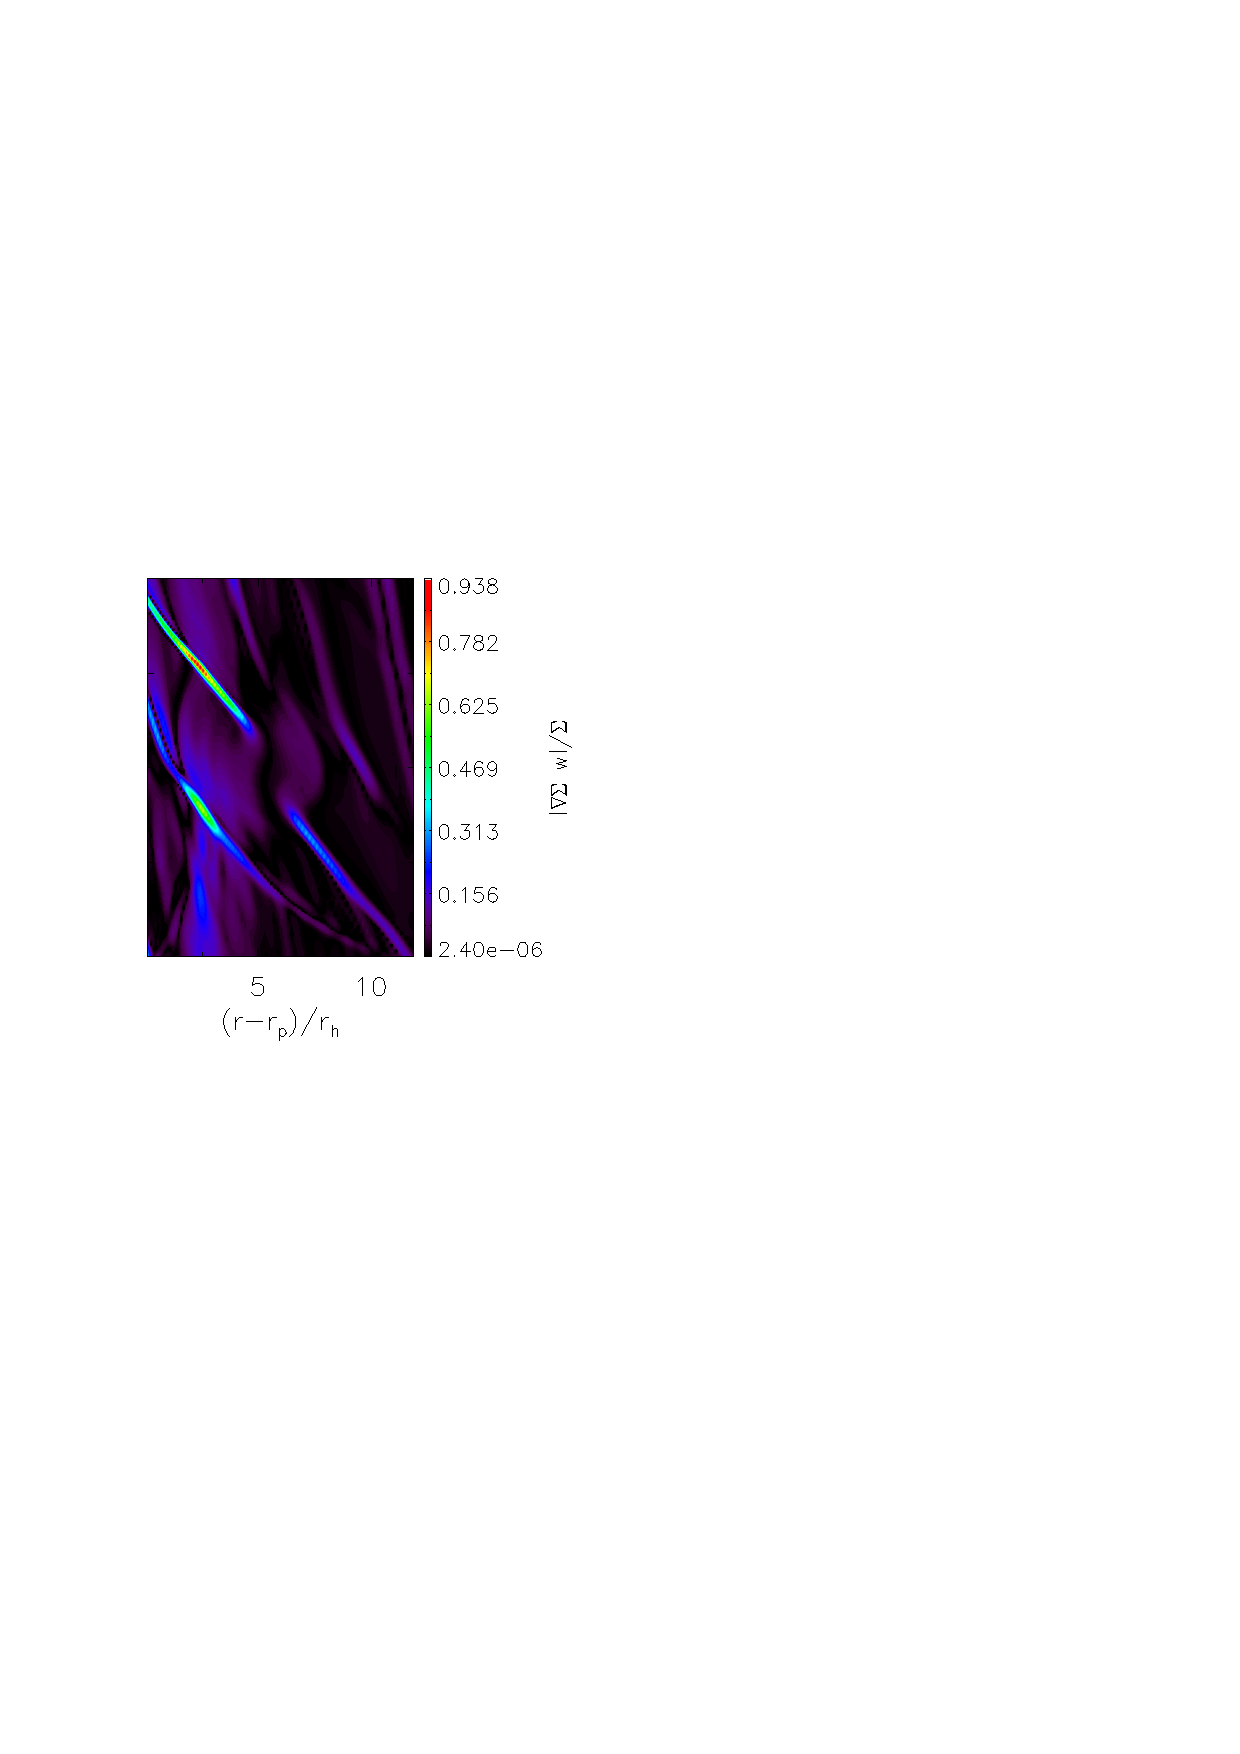
\includegraphics[width=0.3\linewidth]{figures/shock6}
  } 
  \caption{The vortex in the case $\tilde{\beta}=1$
    during quasi-steady state (left), at maximum amplitude of the
    $m=1$ surface density component, 
    (middle), and just after the decay in the $m=1$ amplitude
    (right). The surface density perturbation
    (top) and the associated surface density gradient (bottom) are shown.
    \label{shockplot}}
  % Large surface density gradients become prominant
  % around vortex during dissipation} 
\end{figure}

We also measured large increases in the Mach number near
the vortex as it reaches maximum $m=1$ amplitude and begins to decay. 
Figure \ref{machplot} plots the Mach number $M=|\bm{v} -
\bm{v}_\mathrm{vor}|/c_s$, where 
$\bm{v}_\mathrm{vor}$ corresponds to the bulk velocity of the vortex
around the disc. Values in Fig. \ref{machplot} have been averaged over
a region within $2H$ of the vortex centre. 
During the quasi-steady state the Mach number increase
steadily, and for all cases $M$ reaches a maximum at 
% with larger growth rate for higher $\tilde\beta$.
a time coincident with the start of vortex decay. {\bf check if
  statement is true}

Putting the above observations together, we suggest the decay
in the vortex amplitude is due to shock formation \emph{by the
  vortex}. When the vortex reaches large amplitude, it begins
to induce shocks in the surrounding fluid, as supported by the
increase in Mach number and the appearence of wakes with large surface
density gradients. The vortex may lose energy through shock
dissipation. In addition, a strong vortex (or shock formation) 
can smooth out the gap structure that originally gave rise to the
RWI, which would oppose vortex growth. We examine this below.

\begin{figure}
  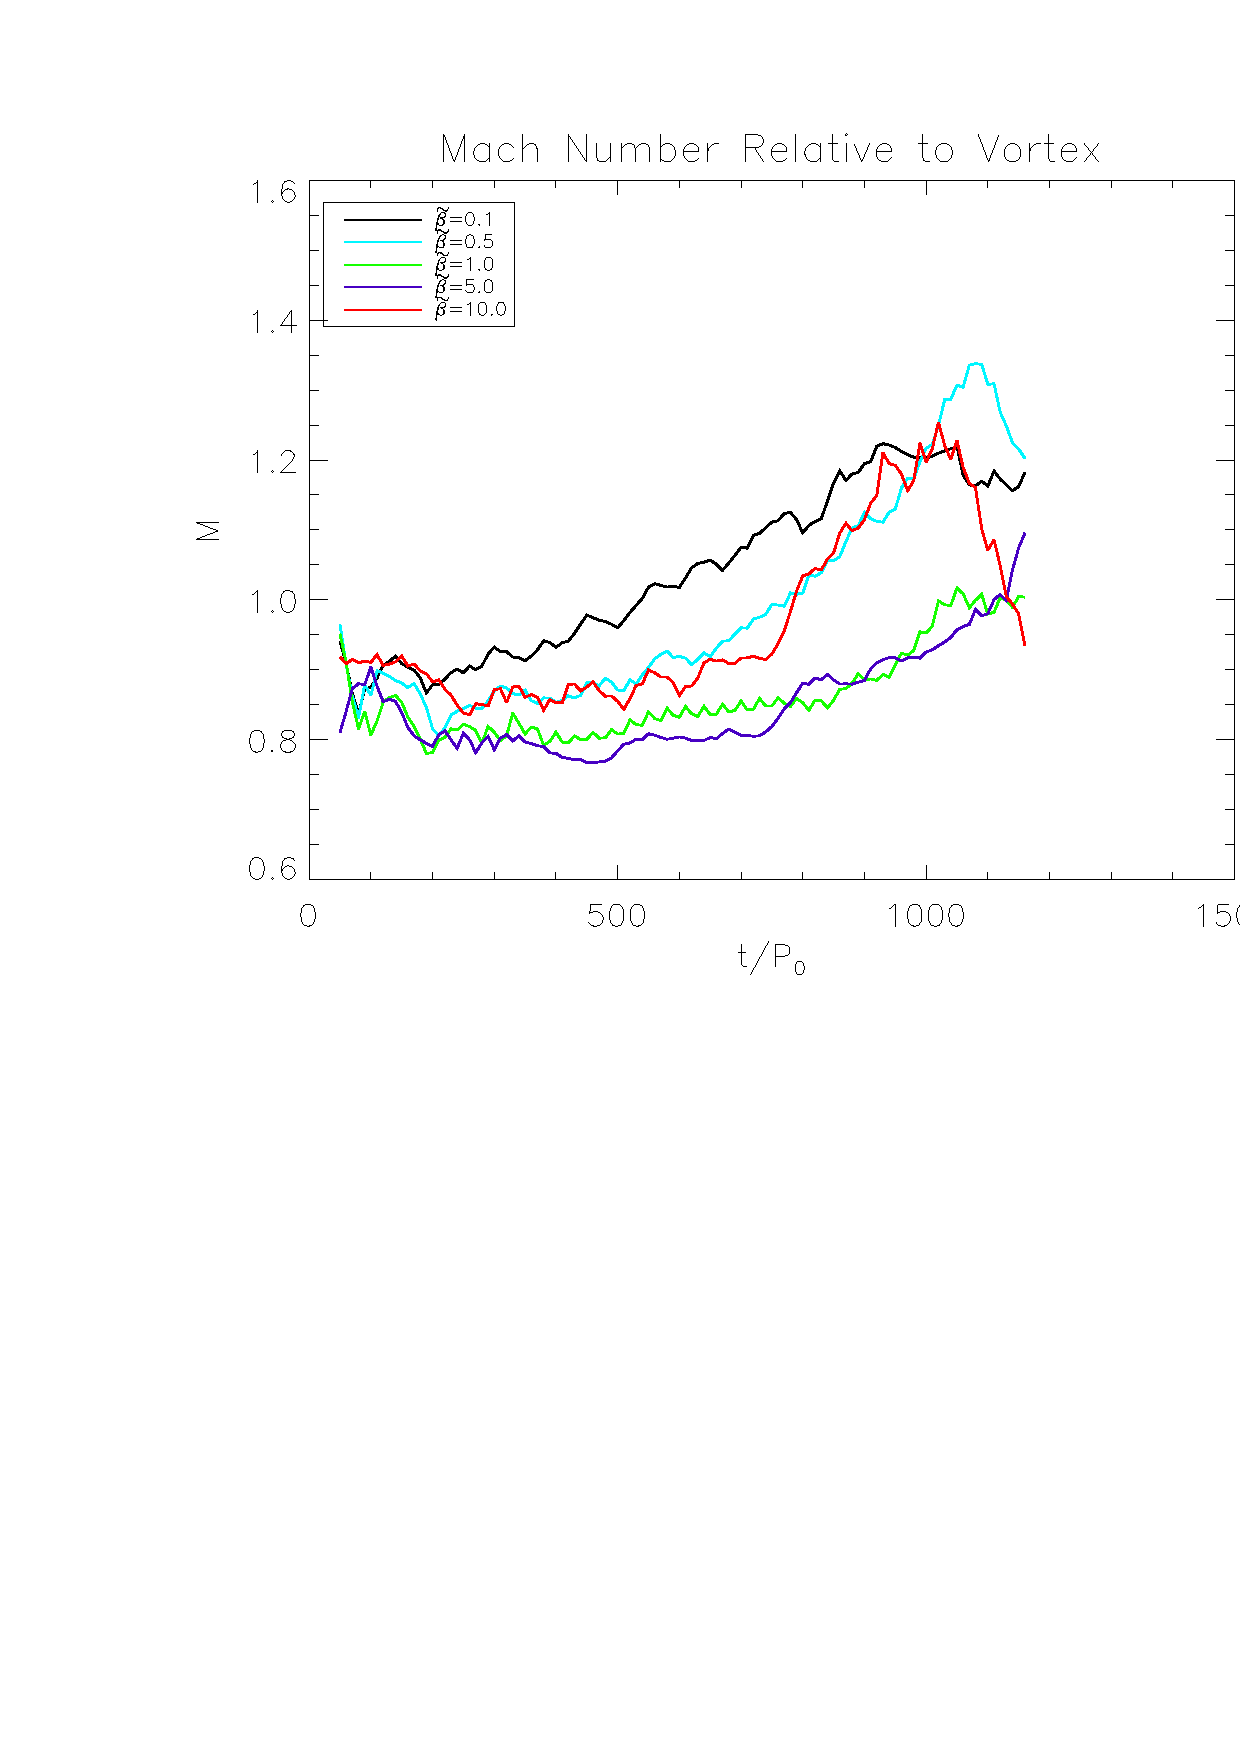
\includegraphics[width=\linewidth]{figures/mach}
  \caption{Running-time average {\bf ?} of the Mach number relative to
    the vortex, averaged over a region within $2H$ of the  
    vortex centre. This plot can be compared to the evolution of the
    vortex amplitude shown in Fig. \ref{lifetimeplot}.
    \label{machplot}}
\end{figure}

\subsection{Vortex decay and gap structure}  
We find vortex decay also modifies the gap
structure. Fig. \ref{gap_smoothed} shows the gap profile before and
after vortex decay for the case $\tilde{\beta}=1$. The vortex resides
around the local surface density maximum at the outer gap edge ($r\sim r_p +
6r_h$). We see that after its amplitude has decayed ($t\sim1500P_0$,   
Fig. \ref{lifetimeplot}), this local surface density maximum is 
smoothed out.           
%and we find that the gap edge is smoothed during this
%process. 
This can be interpreted as the vortex providing a viscosity;  
and we measure a typical alpha viscosity $\alpha = O(10^{-2})$
associated with the vortex. This acts against gap-opening
by the planet, so the condition for the RWI
becomes less favourable, which explains why vortices do not
reform again (at least within the simulation timescale). 
%Thus, the
%time needed for the vortex to grow to sufficient amplitude to modify
%the gap structure  

\begin{figure}
  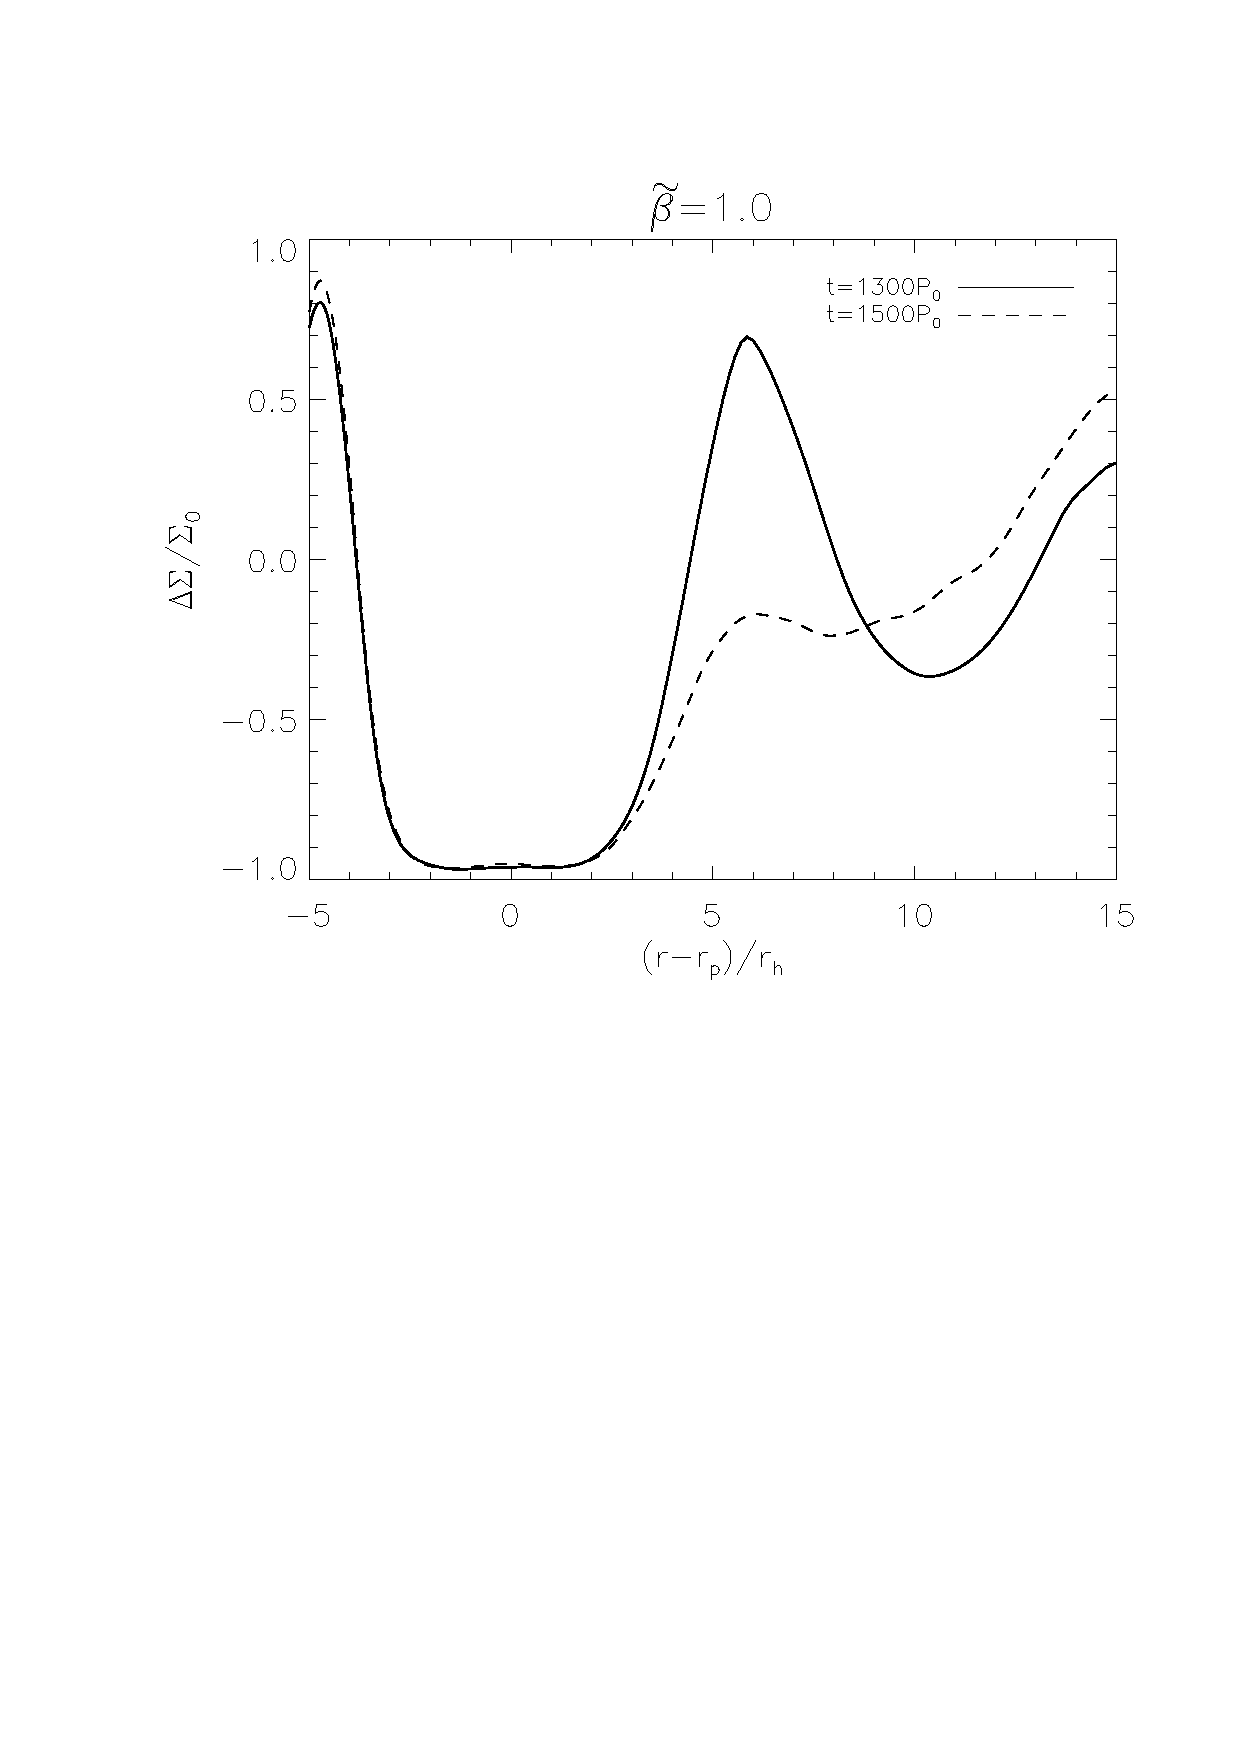
\includegraphics[width=\linewidth]{figures/gapchange}
  \caption{Azimuthally averaged profiles of the relative surface
    density perturbations for  $\tilde\beta=1.0$
    before (solid) and after vortex decay
    (dashed). {\bf remember to correct the time quoted in the
      legend} \label{gap_smoothed}}  
\end{figure}

{\bf It's a good idea to display the smoothening of the outer gap
  edge with time. 
  The gap depth parameter correlates
  well with vortex decay, but its sharp decrease in magnitude gives
  the impression that the gap is 
  `filled', which doesn't reflect Fig. \ref{gap_smoothed}. Visually,
  the gap depth is the same, but the local surface density maximum at
  the outer gap edge is smoothed. Perhaps we can come up with another
  way to characterizing the sharpness of the peak? then we can show
  how this peak is smoothed during vortex decay
}

% Here, we are interested in the region
% $r>r_p$ since the vortex is located at the outer gap edge. We 
% define a gap depth parameter by averaging the relative surface density
% perturbation within $r\in[r_p,r_e]$ where $r_{e}$ is defined as the
% outer gap radius such that $\langle\Delta
% \Sigma(r_e)/\Sigma(t=0)\rangle_{\phi}=0$.  A more negative gap depth
% parameter correlates with a steeper gap edge. 

% Fig. \ref{gapdepth} shows the evolution of the gap depth parameter
% for $\tilde\beta=1.0$. The magnitude of the gap depth is seen to 
% slowly increase as vortex reaches its maximum amplutude at
% $t\sim1000P_0$, followed by a sharp decrease coincident with vortex 
% decay.  

% \begin{figure}
%   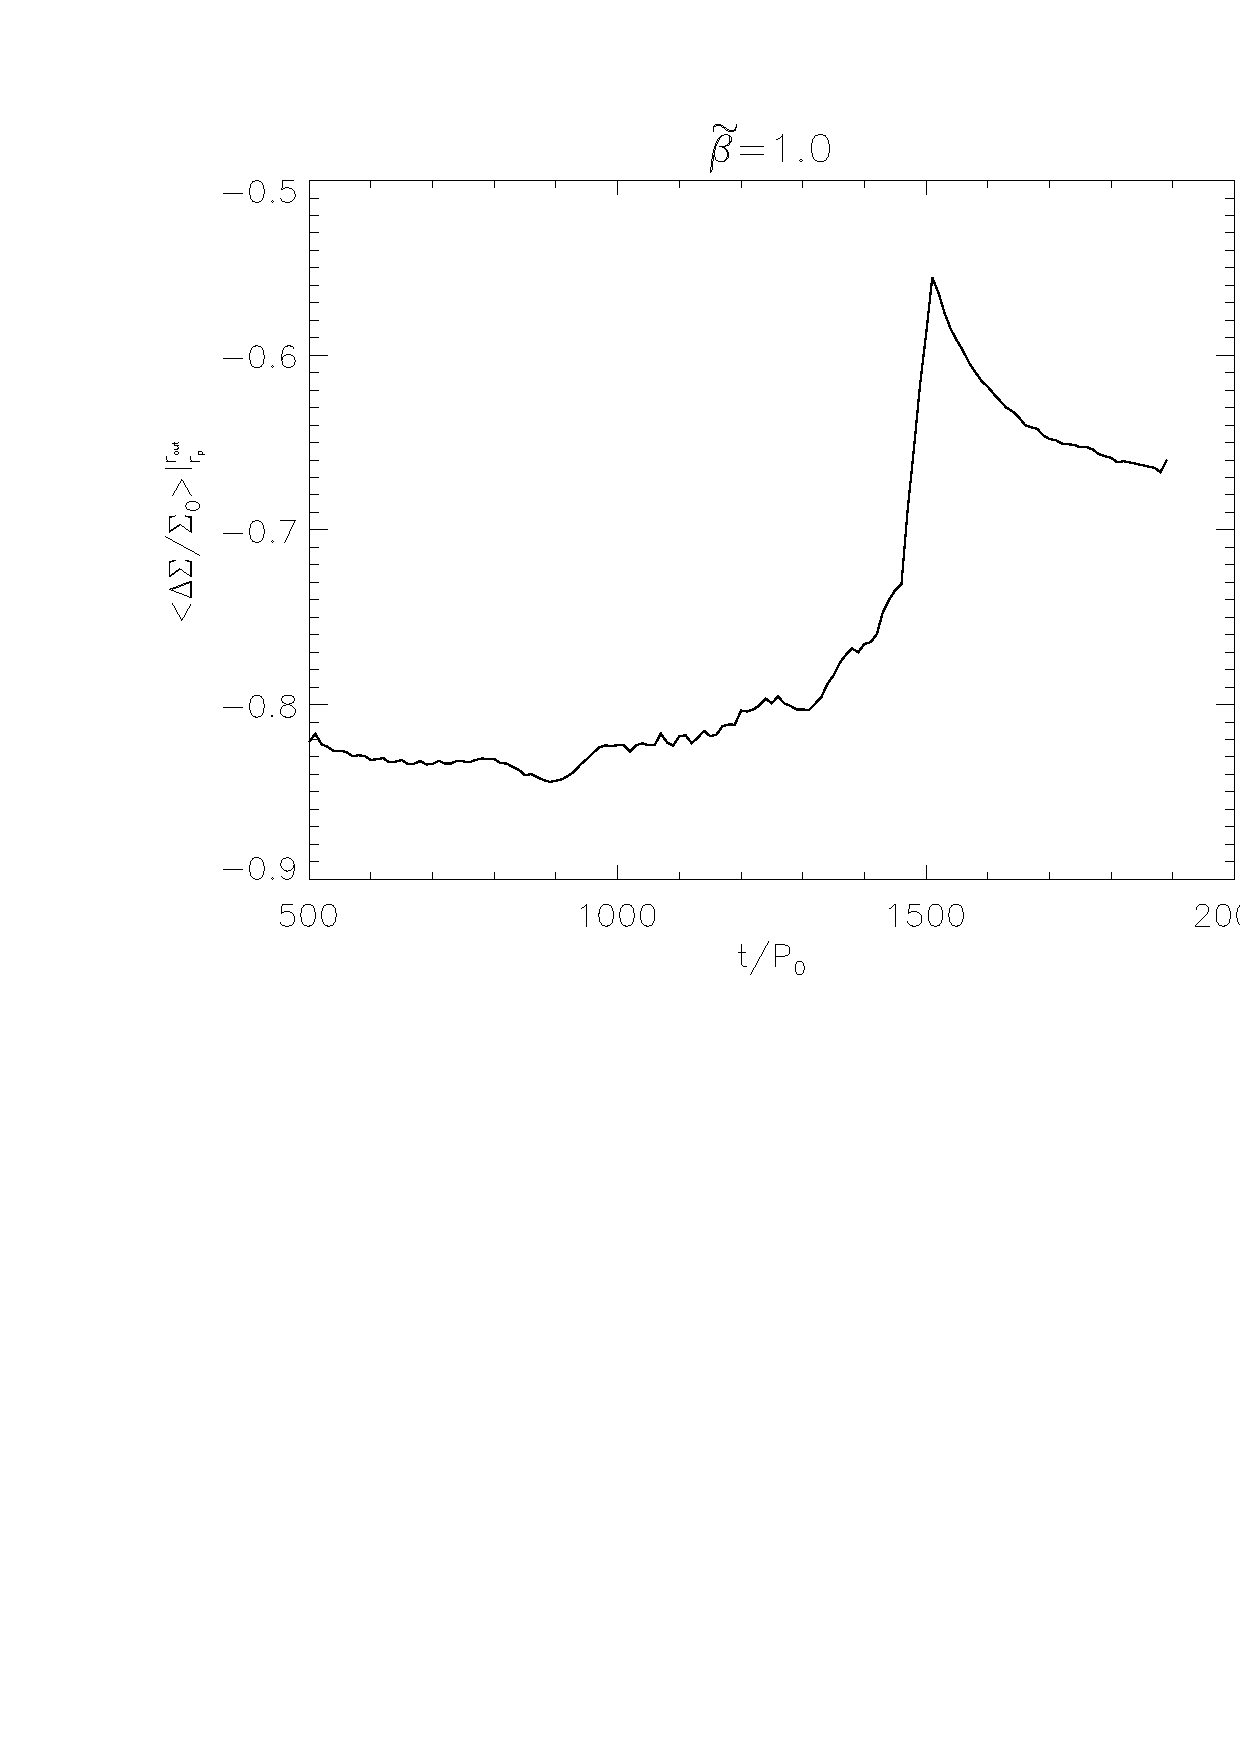
\includegraphics[width=\linewidth]{figures/gapdepth}
%   \caption{Running-time average of the gap depth parameter, defined as
%     the relative surface density perturbation averaged over the
%     outer half of the gap.} \label{gapdepth}
% \end{figure}

\subsection{Vortex lifetimes as a function of cooling
  rate}\label{lifetime_discuss} 
{\bf the discussion here may need to be changed, depending on
  updated/new definitions of vortex lifetime. here, i'm assuming we
  still get the non-monotonic dependence, which may or may not remain
  true. 
}

We now examine vortex lifetimes as function of the imposed cooling
times. We characterise the vortex lifetime as {\bf insert
  definition(s).} and plot this in Fig. \ref{betaplot}. 
Increasing the cooling timescale increases the vortex
lifetime up to $\tilde{\beta}=1$ {\bf (judging from
  Fig. \ref{lifetimeplot} without a quantitative definition)}, after
which vortex lifetimes decrease again. 

%Fig. \ref{lifetimeplot} and Fig. \ref{betaplot} shows that increasing 
%$\tilde{\beta}$
%increases the lifetime of the vortex up to a critical 
%value $\tilde{\beta}=5.0$ for which the vortex lasted to a simulation time of
%$1250P_0$ before starting to dissipate. This is consistent in time with the
%vortex introducing shocks to the system.  

\begin{figure}
  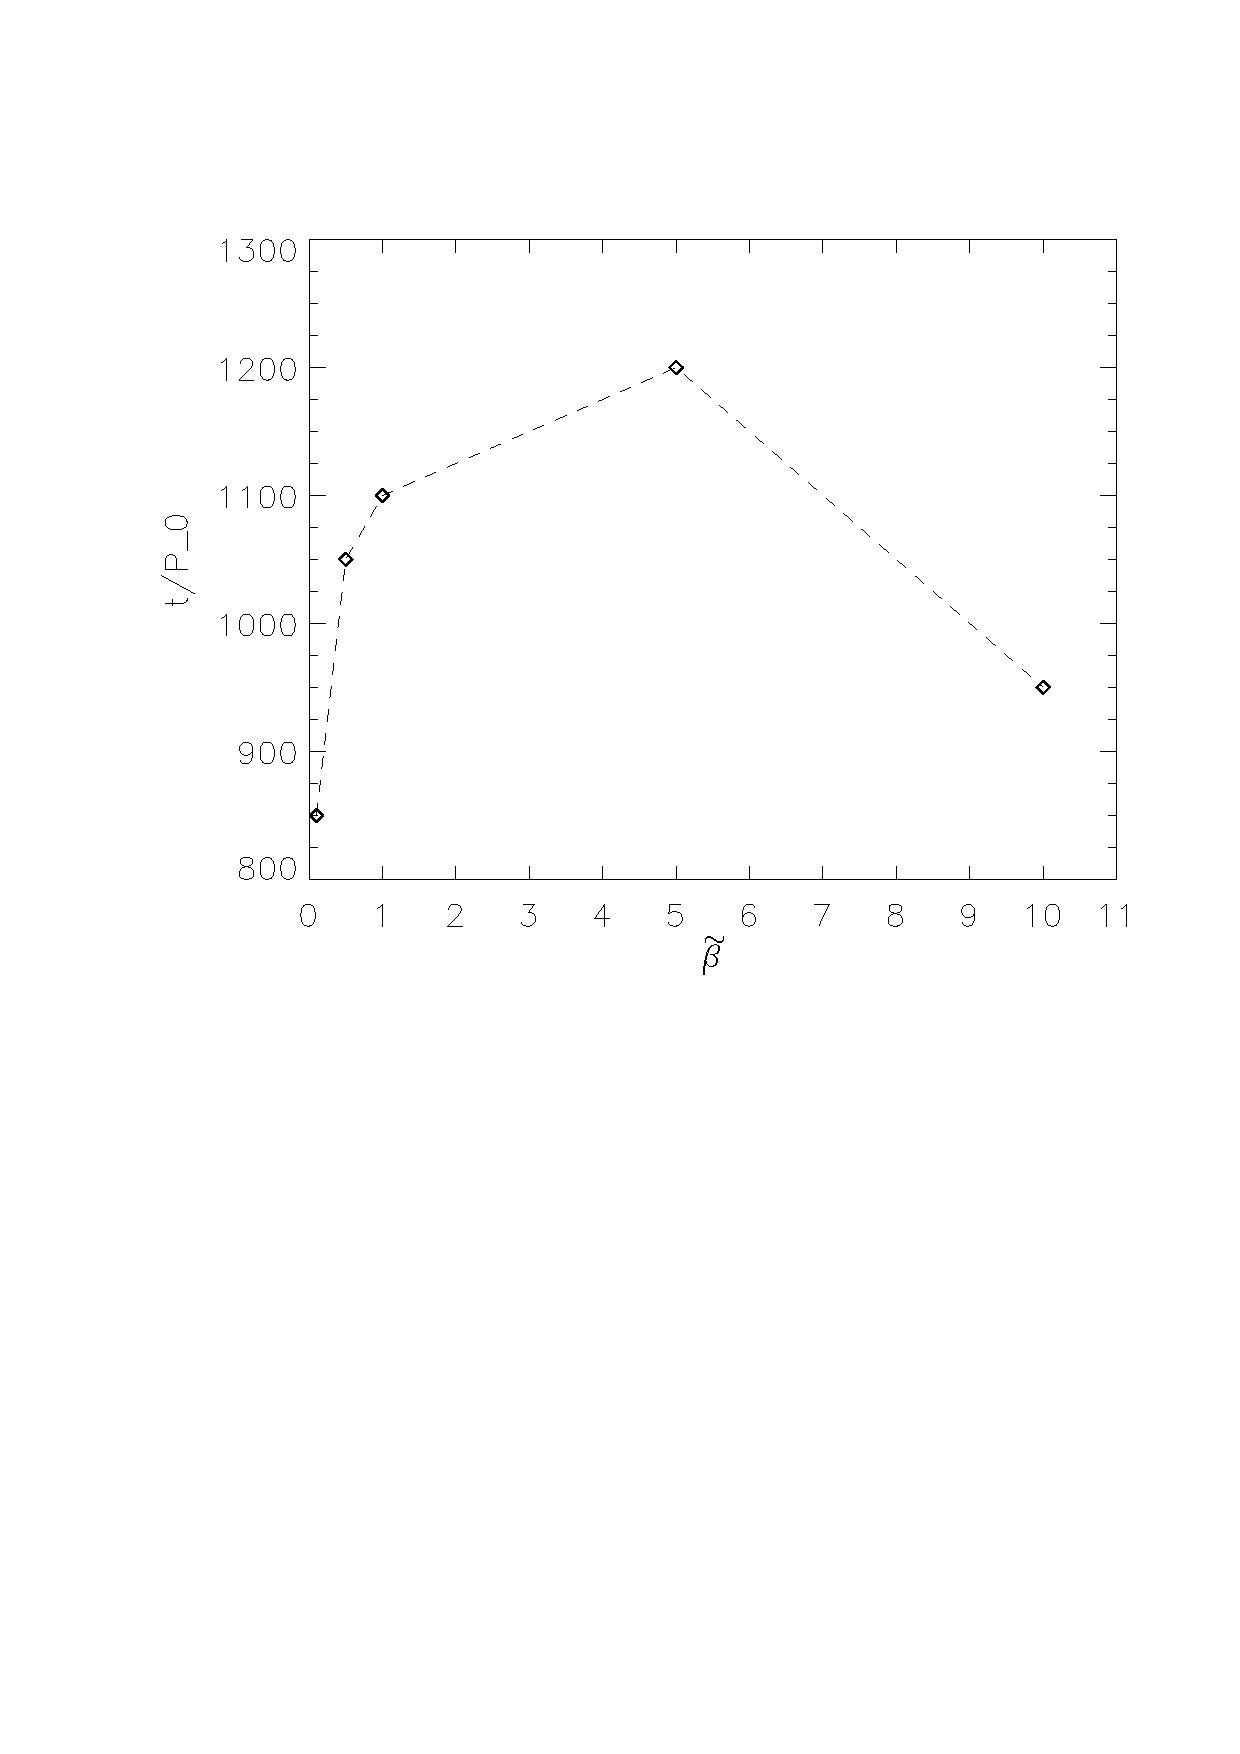
\includegraphics[width=\linewidth]{figures/betaplot}
  \caption{Lifetime of vortices as a function of the cooling paramter 
    $\tilde\beta$. {\bf maybe useful to over-plot other timescales,
      e.g. time taken to reach max mach, time for rossby number to
      reach zero.}\label{betaplot}} 
\end{figure}

In the previous section, we observed that vortices began to decay when
it starts to induce shocks. We therefore suggest that the vortex
timelife is determined by the time needed for the vortex to grow to
sufficient amplitude to induce shocks in the surrounding
fluid. Based on this hypothesis, we suggest below competing
factors that may result in a non-monotonic dependence of vortex
lifetimes on the cooling timescale.  

\subsubsection{Factors contributing to longer vortex lifetimes}
It has been shown that the amplitude at which the RWI saturates 
increases with the growth rate of the linear instability  
\citep{meheut2013}. Our `planet-off' simulations yield slower growth
rates with increasing cooling times, which suggest weaker vortices are
formed initially with increasing $\tilde{\beta}$. This is consistent
with the present simulations: at the beginning of the 
quasi-steady state ($t\sim100P_0$) we find the relative surface density
boost at centre of vortex is $\Delta\Sigma/\Sigma_0=2.5$ for
$\tilde\beta=0.1$ and $\Delta\Sigma/\Sigma_0=1.48$ for
$\tilde\beta=10$.  {\bf rossby numbers?} 

After merging, the growth of the single vortex is mediated by disc-planet
interaction. However, gap-opening becomes more difficult in a hotter 
disc. Furthermore, the increased sound-speed suggest the vortex should    
reach larger amplitudes in order to induce shocks. 

These considerations suggests that, with increased cooling times, 
it takes longer for the vortex grow to sufficient amplitude to induce
shocks and dissipate, implying longer lifetimes with increasing 
$\tilde{\beta}$.      

{\bf hotter disc $\to$ gap edges less sharp, still true during quasi
  steady state?}

\subsubsection{Factors contributing to shorter vortex lifetimes} 
%However, Fig. \ref{lifetimeplot} shows that very long cooling
%times (e.g. $\tilde{\beta}=10$) actually results in a \emph{shorter} vortex
%lifetime. 
Notice in Fig. \ref{lifetimeplot}, for $\tilde{\beta}=10$ the vortex 
growth during the quasi-steady state is in fact faster than for
$\tilde{\beta}=5$. For example, at $t\sim 500P_0$ the vortex with   
$\tilde{\beta}=10$ has the largest amplitude. This is also reflected
in Fig. \ref{machplot}, where the Mach number reaches its maximum
value sooner for $\tilde{\beta}=10$ than for $\tilde{\beta}=5$. 

The above observation is consistent with the RWI being favoured by higher
disc temperatures \citep{li00,lin12c}, which corresponds to longer
cooling times in our case. While our `planet-off' simulations indicate
this is unimportant for the linear instability, it may contribute 
significantly to the vortex growth during quasi-steady state, when one
considers very long cooling times (e.g. $\tilde{\beta}=10$). This
effect alone would lead to a shorter vortex lifetime by allowing it to
induce shocks sooner. 

%This effect can be seen in Mach number around the vortices where the
%growth of Mach number with respect to time is increasing with cooling rate.
%Thus the intially weaker formed vortices for higher cooling rate grow
%substantialy faster than the sound speed and can shock the system in earlier
%times.
%While our `planet-off' simulations show 
%This may be attributed to the higher temperature
%reached in the latter case 
%
%($h\simeq 0.07$) in comparison with the former
%($h\simeq 0.06$), since \cite{li00} showed that the RWI is favoured by
%larger disc temperature.  